\chapter{Data Preparation and Exploratory Analysis}
\label{sec:data_preparation_exploration}

\section{Methodological Objectives}
\label{sec:methodological_objectives}

This chapter establishes the methodological foundation for all subsequent analyses by addressing the construction, organization, and preliminary characterization of the DNA methylation datasets used in this thesis. Following the biological background and problem formulation introduced in Chapters~\ref{chap:introduction} and~\ref{chap:biological_background}, the present chapter acts as a bridge between domain-specific knowledge and quantitative modeling, ensuring that downstream analyses are grounded on a technically sound and well-understood data representation.

Genome-wide DNA methylation data are characterized by extremely high dimensionality, heterogeneous signal-to-noise ratios, and the coexistence of subtle biological effects with multiple sources of technical variability. In this context, premature application of statistical models or feature-selection procedures may lead to biased conclusions driven by artefacts rather than genuine biological structure. A careful examination of data quality, distributional properties, and internal consistency is therefore a necessary prerequisite for any reliable inference \cite{Yousefi2013}.

The primary objective of this chapter is to construct a coherent and reproducible representation of the available datasets and to assess their structural and statistical properties prior to any form of preprocessing or modeling. Specifically, this chapter aims to: (i) describe the organization of methylation matrices and associated phenotype information; (ii) characterize the global and local variability of methylation levels within each dataset; (iii) evaluate the degree of separation between Normal, Adjacent, and Tumor tissues using exploratory tools; and (iv) compare datasets at an inter-cohort level to assess consistency, heterogeneity, and potential limitations in signal transferability.

The scope of this chapter is deliberately restricted to exploratory and diagnostic analyses. No feature selection, predictive modeling, or formal statistical inference is performed at this stage. All analyses are intended to be descriptive and comparative, serving to highlight structural properties of the data and to identify potential technical or biological issues that must be addressed before proceeding further.

Methodologically, the chapter is organized around a unified exploratory framework applied consistently across all datasets. Intra-dataset analyses are used to investigate internal structure, variability patterns, and group-level behavior, while inter-dataset comparisons focus on assessing cross-cohort consistency and platform-related differences. Throughout the chapter, visualizations and summary metrics are employed as diagnostic tools rather than as decision-making instruments.

The results of this exploratory phase reveal both shared characteristics and dataset-specific behaviors, as well as clear limitations of working directly with raw or minimally processed methylation data. These observations motivate the need for a structured and rigorous data pre-processing pipeline, which is developed and justified in the following chapter. The present chapter therefore provides the conceptual and technical basis for the preprocessing choices adopted in Chapter~4 and for all subsequent modeling steps.

\section{Dataset Construction, Metadata Integration, and Data Organization}

This section provides the methodological framework for the selection, construction of the dataset, and the organisation process adopted in this study. It contextualises the data sources, representation choices, metadata management, and computational design principles that underpin the detailed implementation described in the following sections.

\subsection{Data Sources and Study Design}

All datasets analyzed in this thesis were obtained from the NCBI Gene Expression Omnibus (GEO)~\cite{GEO_NCBI}, which was selected as a unified data source to minimize heterogeneity in data formats, metadata conventions, and access mechanisms. GEO provides curated series-level accessions, stable sample identifiers, and standardized links to processed methylation matrices and sample-level annotations, making it a natural reference repository for large-scale DNA methylation studies.

The study design adopts a multi-cohort comparative framework focused on genome-wide DNA methylation in breast tissue. Three independent GEO series were selected for analysis: \textbf{GSE69914}~\cite{GSE69914}, based on the Illumina HumanMethylation450 platform, and two more recent EPIC-based cohorts, \textbf{GSE225845}~\cite{GSE225845} and \textbf{GSE287331}~\cite{GSE287331}. Together, these datasets span normal/healthy, adjacent-normal, and tumor tissue states across two generations of Illumina methylation arrays (450K and EPIC), enabling both within-dataset characterization and cross-dataset comparisons.

Dataset selection was driven by strict inclusion criteria aimed at ensuring technical compatibility, biological relevance, and analytical feasibility. In particular, only studies providing processed genome-wide methylation matrices in terms of $\beta$-values were considered, allowing a uniform data representation and avoiding the need for low-level signal reprocessing from raw \texttt{.idat}  intensity files. Raw \texttt{.idat} files store probe-level fluorescence intensities measured in the methylated ($y^{(M)}$) and unmethylated ($y^{(U)}$) channels, from which $\beta$-values are derived as a normalized ratio \cite{Du2010}:
\begin{equation}
\beta := \frac{\max(y^{(M)},0)}{\max(y^{(M)},0)+\max(y^{(U)},0)+\alpha},
\qquad \beta\in[0,1].
\label{eq:beta_definition}
\end{equation}
where $\alpha$ is a small offset (typically 100) used to stabilize the denominator. Additional requirements included the use of Illumina HumanMethylation450 (450K) or MethylationEPIC (EPIC) platforms, the availability of multiple tissue classes within each cohort, and sufficiently large sample sizes to support robust statistical analysis.

\subsection{Methylation Data Representation and Storage}

In several datasets, the original authors applied established normalization procedures, including methods specifically designed to correct probe-type design bias such as BMIQ~\cite{Teschendorff2013BMIQ}. Reprocessing raw IDAT files would therefore not add information relevant to the objectives of this thesis, while substantially increasing technical complexity and reducing reproducibility. For these reasons, all analyses were conducted on the processed $\beta$-value matrices as distributed via GEO.

To support scalable analysis and efficient input/output operations, all working methylation matrices were converted to a standardized \texttt{sample~$\times$~CpG} layout and stored in columnar Parquet format using single-precision floating-point encoding.

This choice is motivated by both numerical and computational considerations. Since $\beta$-values are strictly bounded in the interval $[0,1]$~\cite{Du2010}, and biologically meaningful methylation differences typically occur at magnitudes on the order of $10^{-2}$–$10^{-3}$, single-precision floating point (\texttt{float32}, machine $\varepsilon \approx 10^{-7}$) provides more than sufficient numerical accuracy. At the same time, it substantially reduces memory usage and I/O overhead compared to double precision.

This representation is consistent with recent large-scale genomics frameworks that process molecular features, including DNA methylation data, entirely in \texttt{float32} precision for efficiency and scalability~\cite{deAlmeida2025ChatNT}.

\subsection{Phenotype Tables and Label Harmonization}

For each dataset, a dedicated phenotype table was constructed by extracting and parsing GEO sample-level metadata. These tables encode tissue labels, sample identifiers, and relevant clinical or technical covariates when available. Given the heterogeneity of original annotations across studies, tissue classes were mapped to harmonized numeric encodings to ensure consistency across cohorts while preserving dataset-specific attributes in separate fields.

A strict one-to-one correspondence between methylation matrices and phenotype tables was enforced. Samples lacking either methylation measurements or corresponding metadata were excluded to prevent inconsistencies and downstream misalignment. This design guarantees that all analyses operate on synchronized molecular and phenotypic representations and enables reliable stratification by tissue class in both intra- and inter-dataset comparisons.

\subsection{Reproducibility and Computational Workflow}

The overall data organization and computational design follow a multi-dataset analytical paradigm commonly adopted in recent large-scale DNA methylation studies, in which cohort-specific analyses are complemented by cross-dataset comparisons to explicitly evaluate robustness and generalizability, while simultaneously revealing cohort-dependent effects and limitations in signal transferability that motivate subsequent methodological refinement~\cite{Sokolov2024}.

All dataset construction and organization steps were implemented using deterministic, script-based pipelines with explicit schema definitions and typed data representations. Particular care was taken to avoid unnecessary in-memory operations on high-dimensional methylation matrices, favoring streaming ingestion, chunked processing, and out-of-core transformations when required by dataset size.

The resulting data organization yields a set of standardized, self-contained datasets, each consisting of a genome-wide methylation matrix and an aligned phenotype table stored in efficient, portable formats. This design ensures full reproducibility of the data preparation process and provides a robust foundation for the preprocessing, exploratory analysis, and modeling steps developed in subsequent chapters.

\section{Intra-Dataset Exploration and Visualization}
\label{sec:intra_dataset}

This section presents a structured intra-dataset exploratory analysis aimed at characterising the internal statistical and biological organisation of each methylation cohort prior to any preprocessing or modelling step. Each dataset is analysed independently in order to assess data integrity, quantify variability patterns, and evaluate whether Normal, Adjacent, and Tumor tissues exhibit distinguishable epigenetic behaviour.

In the context of breast cancer, epigenetic deregulation is known to manifest through both global and local phenomena, including genome-wide hypomethylation, focal hypermethylation of tumour-suppressor regions, and the presence of pre-neoplastic ``field defects'' in histologically normal tissues proximal to tumours \cite{ehrlich2002, bird2002, teschendorff2016}. These mechanisms motivate an exploratory investigation focused not only on overt tumour-associated changes, but also on more subtle alterations in Normal and Adjacent samples, which are central to the biological hypothesis of this thesis.

This section therefore applies a unified exploratory framework to each dataset (GSE69914 [\ref{subsec:gse69914}], GSE225845 [\ref{subsec:gse225845}], GSE287331 [\ref{subsec:gse287331}]), systematically examining data quality, global methylation distributions, sample-level summaries, CpG-wise variability and instability, correlation structure, dimensionality reduction, and genomic context coverage. The use of a consistent analytical protocol enables direct comparison of intra-dataset behaviour while preserving cohort-specific characteristics.

% ============================================
% 2.1 GSE69914
% ============================================
\subsection{Dataset GSE69914}
\label{subsec:gse69914}

\begin{table}[t]
\centering
\caption{Overview of the GSE69914 dataset after initial cohort curation.}
\label{tab:gse69914_overview}
\scriptsize
\begin{tabular}{c c c c c c c}
\toprule
\textbf{CpGs} &
\textbf{Samples} &
\textbf{Normal} &
\textbf{Adjacent} &
\textbf{Tumor} &
\textbf{Normal (BRCA1)} &
\textbf{Tumor (BRCA1)} \\
\midrule
485{,}512 &
407 &
50 &
42 &
305 &
3 &
7 \\
\bottomrule
\end{tabular}
\end{table}

\paragraph{Dataset overview}
\label{par:gse69914_overview}

GSE69914 is a breast tissue DNA methylation cohort profiled using the Illumina Infinium HumanMethylation450 BeadChip, providing genome-wide coverage of approximately $4.8\times10^5$ CpG loci. The dataset comprises samples spanning the full Normal--Adjacent--Tumor spectrum that motivates the biological framework of this thesis.

An overview of the sample composition and CpG coverage is reported in Table~\ref{tab:gse69914_overview}, including the distribution across tissue classes and hereditary-risk subgroups.

A limited subset of samples is associated with germline \textit{BRCA1} mutations. \textit{BRCA1}, in particular, encodes a key DNA repair protein, and pathogenic variants are known to substantially increase lifetime breast and ovarian cancer risk \cite{brca_factsheet}. Multiple studies have shown that BRCA-associated breast tissues exhibit distinct baseline epigenetic profiles, reflecting inherited genomic instability rather than sporadic tumorigenesis \cite{Bartlett2022,Suijkerbuijk2008}.

Since the primary objective of this thesis is to characterise early, field defect DNA methylation alterations along the Normal--Adjacent axis in sporadic breast cancer, samples carrying \textit{BRCA1} mutations were excluded from the core exploratory and preprocessing pipeline. Their inclusion would introduce a confounding hereditary epigenetic signal, potentially obscuring subtle methylation shifts in non-mutated normal and adjacent tissues.




% ============================================
% Beta distributions
% ============================================

\paragraph{Global methylation distributions}
\label{par:gse69914_global_meth}

To characterise the overall methylation landscape of the dataset, the distribution of $\beta$-values
(fractional methylation in $[0,1]$) was first examined.
The group-wise mean density curve (Figure~\ref{fig:gse69914_group_mean_density}) displays the
characteristic \emph{bimodal} profile of Illumina 450k arrays, with peaks near unmethylated
($\beta \approx 0$) and fully methylated ($\beta \approx 1$) CpG sites. This pattern reflects
the underlying biology of CpG regulation, where many loci tend to be either transcriptionally
active (hypomethylated) or repressed (hypermethylated) \cite{bird2002, maksimovic2012}.

When comparing tissue groups, a clear gradient emerges.
Tumor samples show a slightly flatter high-$\beta$ peak and a broader low-$\beta$ tail,
consistent with the well-described phenomenon of global hypomethylation and increased
heterogeneity in cancer \cite{ehrlich2002}. Adjacent samples lie between Normal and
Tumor, suggesting early epigenetic drift and subtle field defects occurring in histologically
non-neoplastic tissue \cite{teschendorff2016}.

\begin{figure}[t]
    \centering
    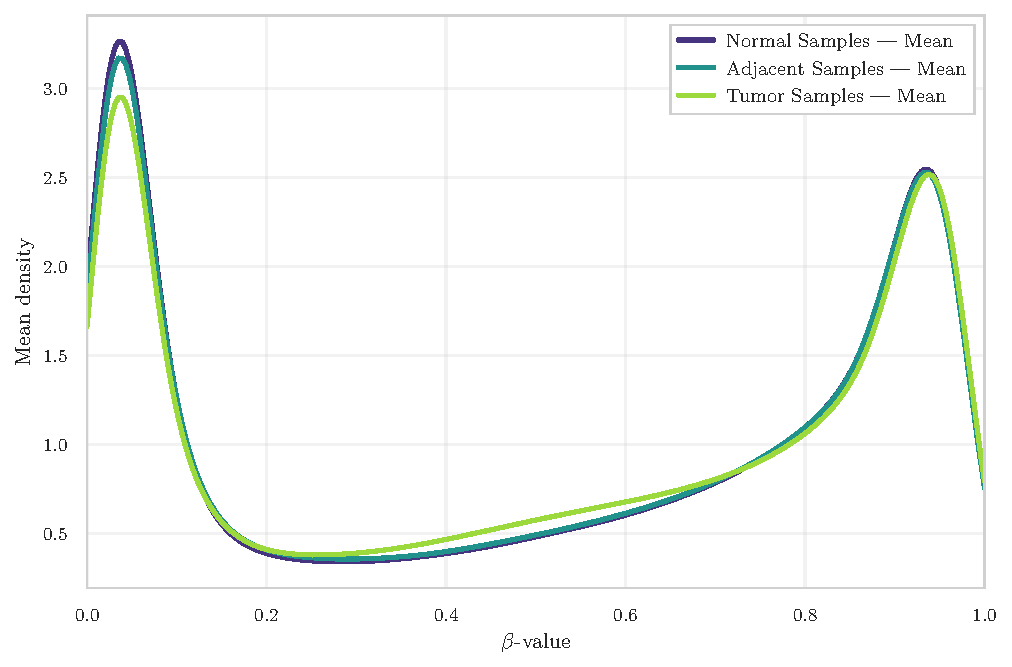
\includegraphics[width=0.5\linewidth]{images/cap3/GSE69914_04_beta_density_group_mean.pdf}
    \caption{Group-wise mean $\beta$-value density in GSE69914.}
    \label{fig:gse69914_group_mean_density}
\end{figure}



% ============================================
% Outlier burden
% ============================================

\paragraph{CpG-level instability and recurrent outliers}
\label{par:gse69914_outliers}

To characterise locus-specific instability, the 200 CpG sites with the highest
outlier burden across samples were examined. The heatmap of the top outlier loci
(Figure~\ref{fig:gse69914_outliers_heatmap}) indicates that epigenetic disruption is
\emph{not uniform}: specific CpG sites and specific samples display extreme deviations,
rather than a diffuse genome-wide shift. Moreover, both directions of alteration are
present — focal hypermethylation and focal
hypomethylation.
In cancer biology, hypermethylation can silence tumor-suppressor regions, whereas
hypomethylation can derepress oncogenic pathways and weaken genomic stability, reflecting
the classic “too much and too little methylation’’ behaviour of tumor genomes
\cite{ehrlich2002}.

Complementary $\Delta\beta$ distributions comparing Tumor and Adjacent tissues against Normal
(Figure~\ref{fig:gse69914_outliers_deltabeta}) show a clear shift toward
hypomethylation in Tumor samples and a subtler but detectable drift in Adjacent tissues.
This provides evidence that epigenetic alterations emerge early in histologically normal
tissue located near the tumor, supporting the field-cancerization model
\cite{teschendorff2016}.

\begin{figure}[t]
    \centering
    \begin{subfigure}[t]{0.48\linewidth}
        \centering
        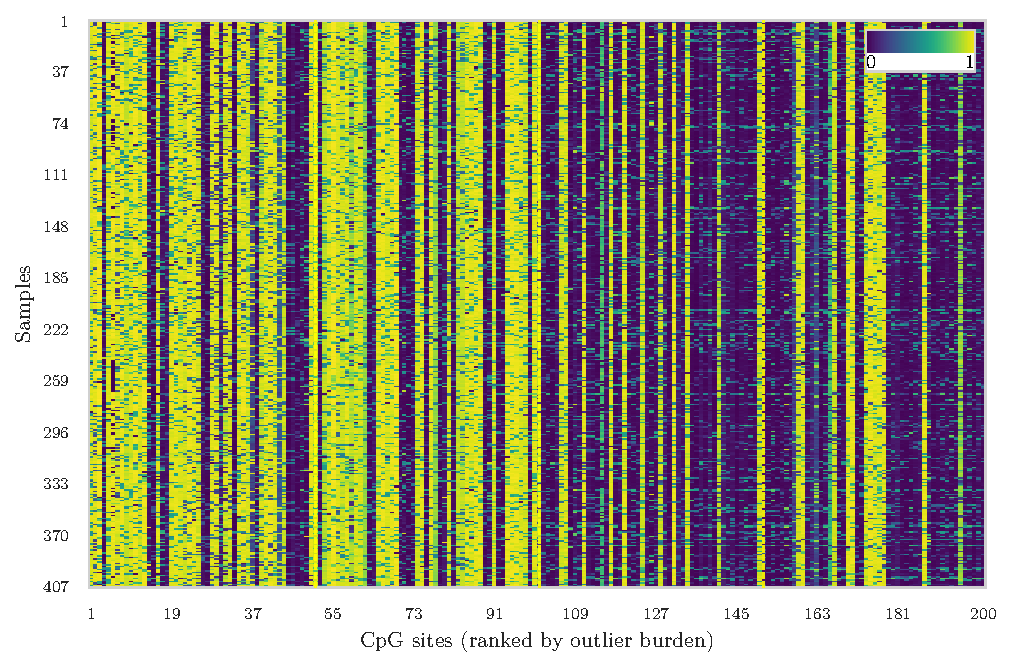
\includegraphics[width=\linewidth]{images/cap3/GSE69914_11_heatmap_top_outlier_cpgs_numbered.pdf}
        \caption{Top outlier CpG loci.}
        \label{fig:gse69914_outliers_heatmap}
    \end{subfigure}
    \hfill
    \begin{subfigure}[t]{0.48\linewidth}
        \centering
        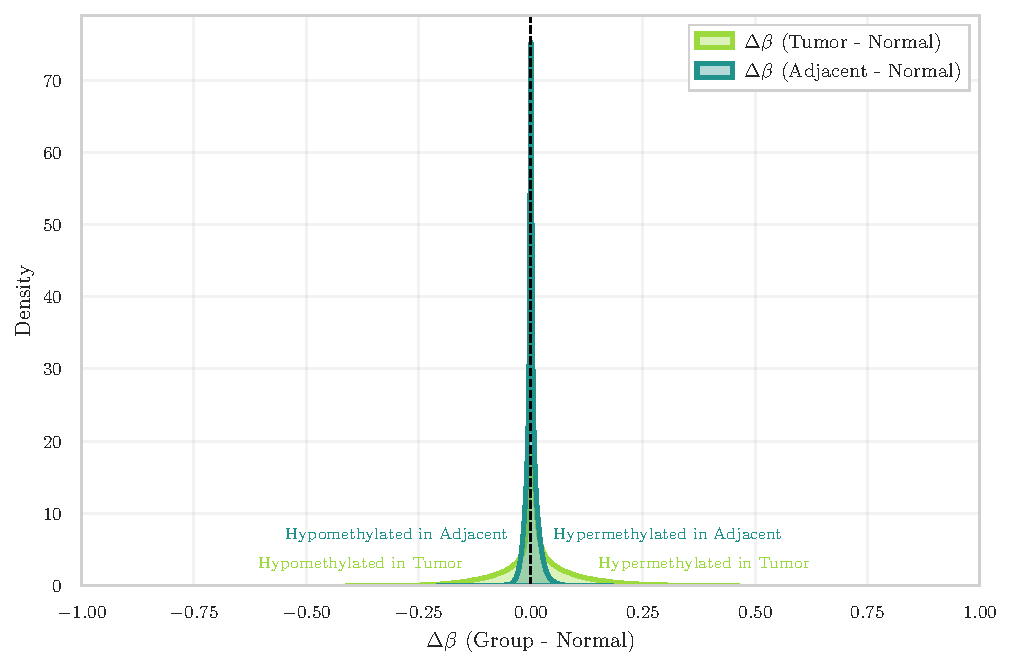
\includegraphics[width=\linewidth]{images/cap3/GSE69914_12_delta_beta_overlaid.pdf}
        \caption{$\Delta\beta$ distributions (Tumor/Adjacent $-$ Normal).}
        \label{fig:gse69914_outliers_deltabeta}
    \end{subfigure}
    \caption{Heatmap of the top outlier CpGs (left) and corresponding $\Delta\beta$ distributions (right), illustrating CpG-level instability in GSE69914.}
    \label{fig:gse69914_outliers_combined}
\end{figure}


% ============================================
% Variance, correlation, moments
% ============================================
\paragraph{Variance and correlation structure}
\label{par:gse69914_variance_corr}
To quantify within-group epigenetic variability, the distribution of CpG-wise
variance across samples was examined. The density curves
(Figure~\ref{fig:gse69914_var_corr_variance}) show that Tumor samples have markedly
higher variance, reflecting increased epigenetic instability.
In contrast, Normal and Adjacent samples display almost identical variance
distributions that are tightly concentrated near zero.
This indicates that, at the level of CpG-wise variability, Adjacent tissues do not yet
exhibit detectable divergence from Normal samples.

A complementary perspective is provided by the sample correlation heatmap
(Figure~\ref{fig:gse69914_var_corr_correlation}), which shows the expected high level of
pairwise similarity across all samples. This behaviour is typical of genome-wide DNA
methylation data, where a large fraction of CpG sites is stable across individuals,
resulting in consistently strong correlations \cite{Teschendorff2013BMIQ}.
Importantly, the heatmap also reveals that all samples are highly mutually correlated,
with no sharp blocks or boundaries separating the three tissue labels. This confirms that
global methylation structure is largely conserved across Normal, Adjacent and Tumor tissues,
and that group differences are too subtle to be detected through
sample–sample correlation alone.

\begin{figure}[t]
    \centering
    \begin{subfigure}[t]{0.48\linewidth}
        \centering
        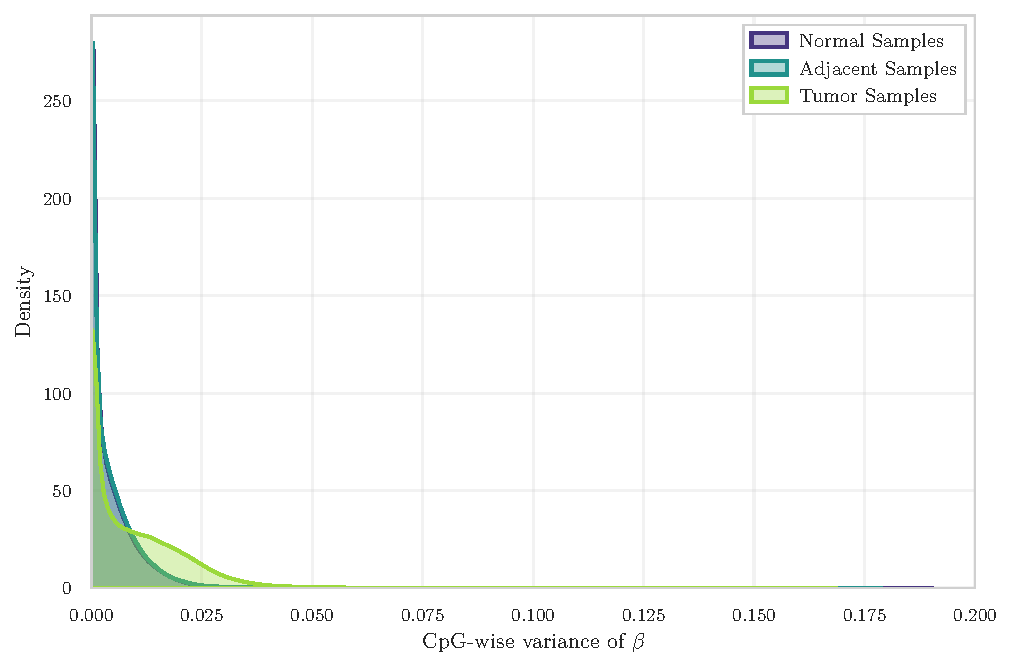
\includegraphics[width=\linewidth]{images/cap3/GSE69914_13_intragroup_variance.pdf}
        \caption{CpG-wise variance distributions.}
        \label{fig:gse69914_var_corr_variance}
    \end{subfigure}
    \hfill
    \begin{subfigure}[t]{0.48\linewidth}
        \centering
        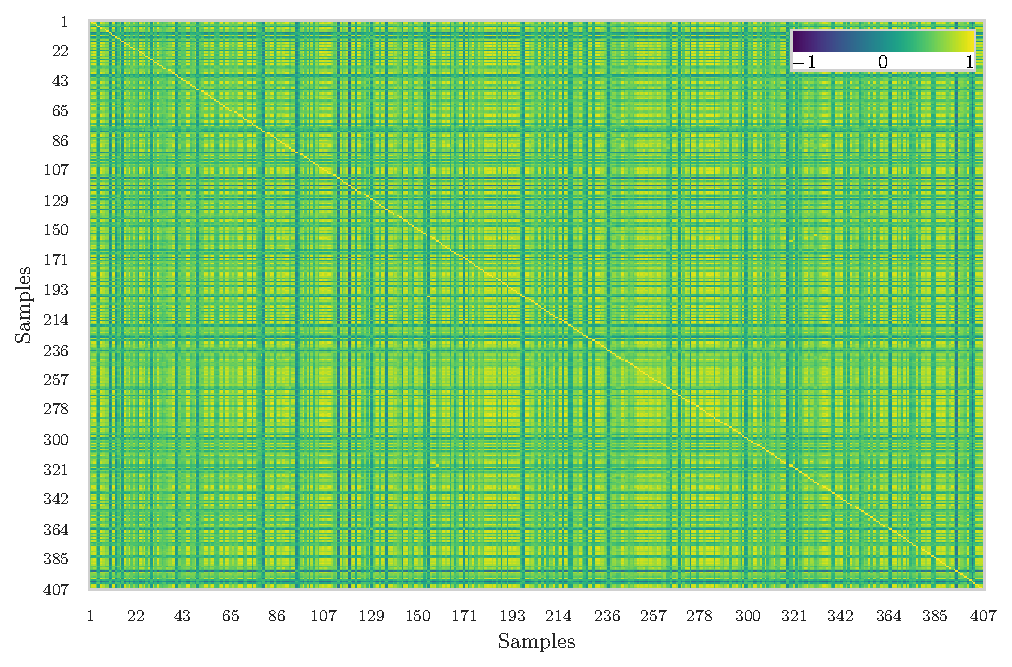
\includegraphics[width=\linewidth]{images/cap3/GSE69914_14_sample_correlation_heatmap.pdf}
        \caption{Sample correlation heatmap.}
        \label{fig:gse69914_var_corr_correlation}
    \end{subfigure}
    \caption{Variance and correlation structure across Normal, Adjacent, and Tumor samples in GSE69914.}
    \label{fig:gse69914_var_corr}
\end{figure}


% ============================================
% DR: PCA, tSNE, UMAP
% ============================================
\paragraph{Low-dimensional embeddings}
\label{par:gse69914_embeddings}

Dimensionality reduction was applied using Principal Component Analysis (PCA),
t-distributed Stochastic Neighbor Embedding (t-SNE), and Uniform Manifold
Approximation and Projection (UMAP) to visualise global similarities among samples
(Figure~\ref{fig:gse69914_embeddings_combined}).
Across all three methods, Normal and Adjacent samples show substantial overlap,
with no clear separation between these two groups. Tumor samples appear more dispersed,
but only mildly shifted relative to the Normal/Adjacent cluster, and no sharp cluster
boundaries emerge in any embedding. The trustworthiness scores are similar across embeddings (0.869–0.888),
indicating that local neighbourhood relationships are largely preserved
in the low-dimensional projections.

These projections indicate that global methylation patterns alone do not
provide strong discriminative structure among the three tissue states. This suggests
that group differences are subtle at the whole-methylome level and are more effectively
captured through locus-specific analyses rather than through global unsupervised embeddings.
\begin{figure}[t]
    \centering
    \begin{subfigure}[t]{0.32\linewidth}
        \centering
        
\includegraphics[width=\linewidth]{images/cap3/GSE69914_16_pca.pdf}
        \caption{PCA \\$\text{trustworthiness}=0.869$.}
    \end{subfigure}
    \hfill
    \begin{subfigure}[t]{0.32\linewidth}
        \centering
        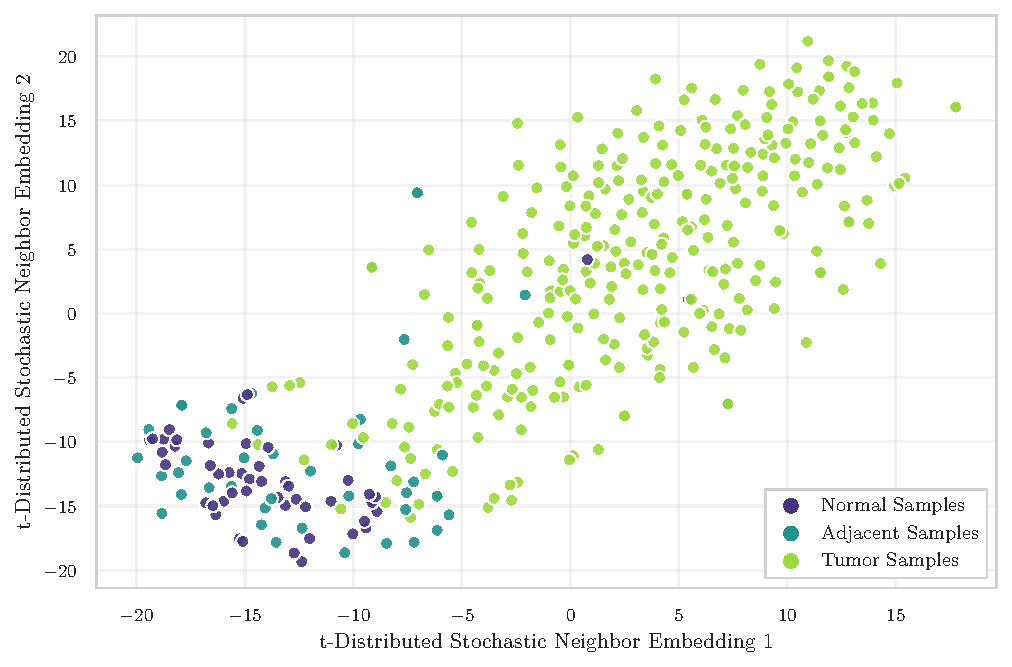
\includegraphics[width=\linewidth]{images/cap3/GSE69914_17_tsne.pdf}
        \caption{t-SNE \\$\text{trustworthiness}=0.888$.}
    \end{subfigure}
    \hfill
    \begin{subfigure}[t]{0.32\linewidth}
        \centering
        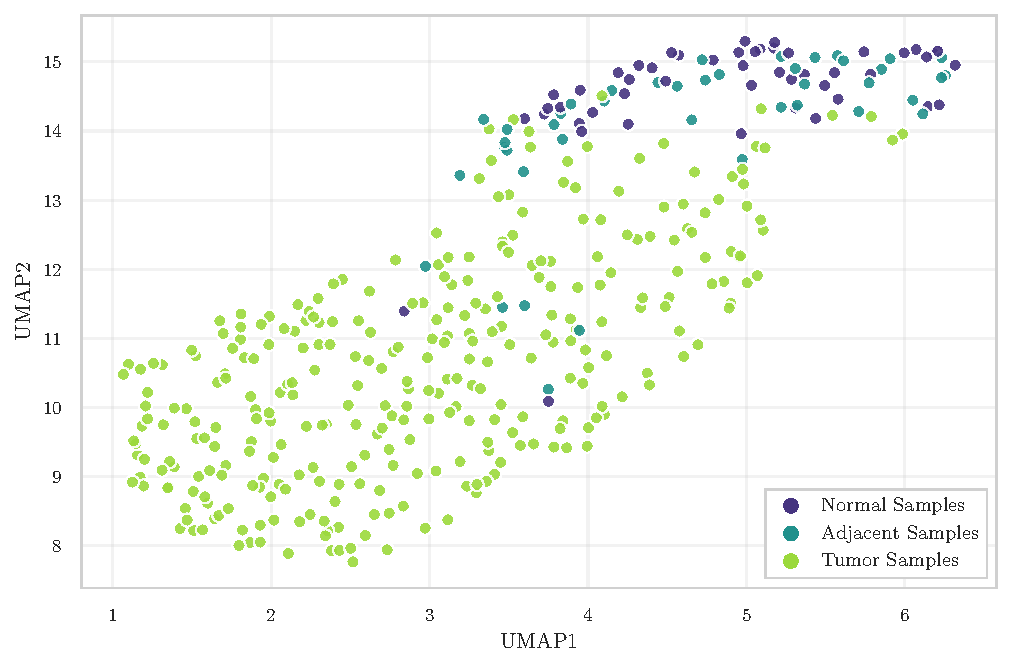
\includegraphics[width=\linewidth]{images/cap3/GSE69914_18_umap.pdf}
        \caption{UMAP \\$\text{trustworthiness}=0.874$.}
    \end{subfigure}
    \caption{Low-dimensional embeddings samples in GSE69914.}
    \label{fig:gse69914_embeddings_combined}
\end{figure}

% ============================================
% Manifest coverage
% ============================================
\paragraph{Genome annotation coverage}
\label{par:gse69914_manifest}

CpG probes were annotated using the official \textit{Infinium MethylationEPIC v1.0 B5}
\cite{illumina_manifest_epic} manifest file, the standard Illumina resource containing
genomic coordinates, probe type, CpG island context (Island, Shore, Shelf, Open Sea),
and gene-level annotations.
Using this manifest, the dataset exhibits the expected non-uniform genomic
distribution of CpG contexts: the largest fraction of probes maps to open-sea or
non-island regions, followed by CpG islands, then north and south shores, and finally
north and south shelves. This ordering mirrors the characteristic architecture of the
HM450 arrays reported in the literature~\cite{zhou2017, pidsley2016}.
The coverage observed is therefore consistent with the known genomic
composition of the Illumina methylation arrays, supporting correct manifest alignment.

% ============================================
% Dynamic network proxies
% ============================================
\paragraph{Dynamic-network proxies}
\label{par:gse69914_dnb_proxies}

\begin{figure}[t]
    \centering
    \begin{subfigure}[t]{0.32\linewidth}
        \centering
        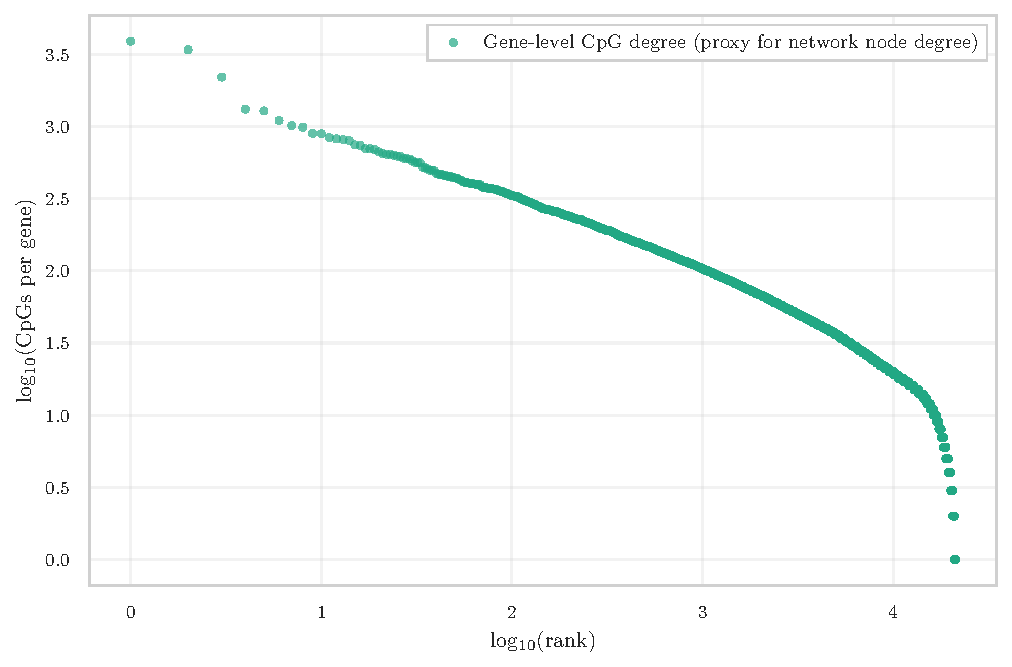
\includegraphics[width=\linewidth]{images/cap3/GSE69914_20_dynamic_network_degree_proxy.pdf}
        \caption{Gene-level CpG degree distribution.}
        \label{fig:gse69914_dnb_degree}
    \end{subfigure}
    \hfill
    \begin{subfigure}[t]{0.32\linewidth}
        \centering
        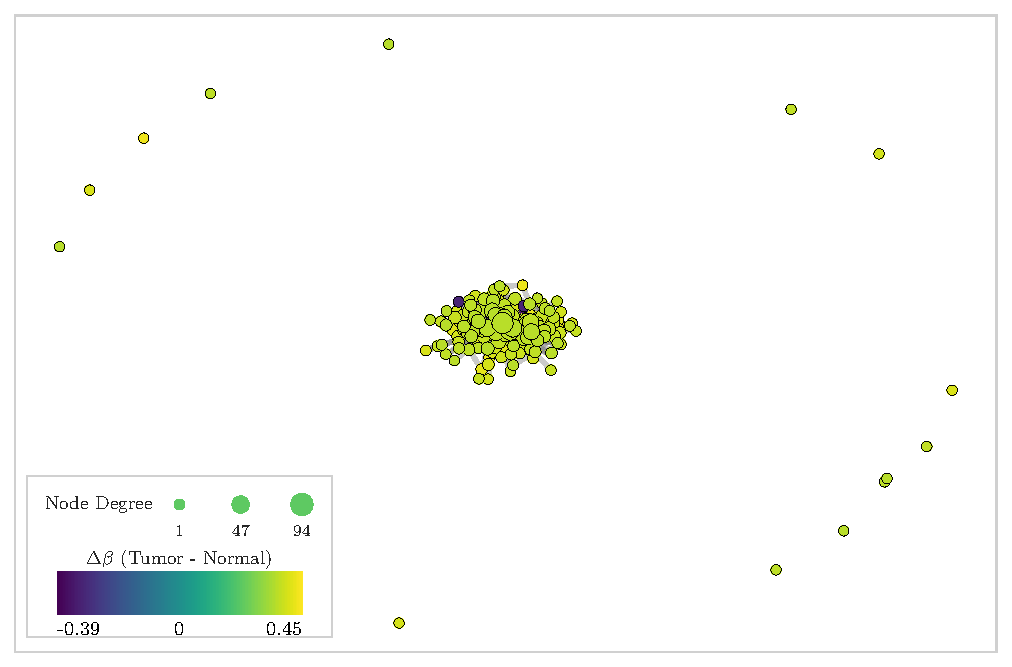
\includegraphics[width=\linewidth]{images/cap3/GSE69914_21_dnb_network_tumor_minus_normal.pdf}
        \caption{DNB-like network: Tumor vs Normal.}
        \label{fig:gse69914_dnb_tumor_normal}
    \end{subfigure}
    \hfill
    \begin{subfigure}[t]{0.32\linewidth}
        \centering
        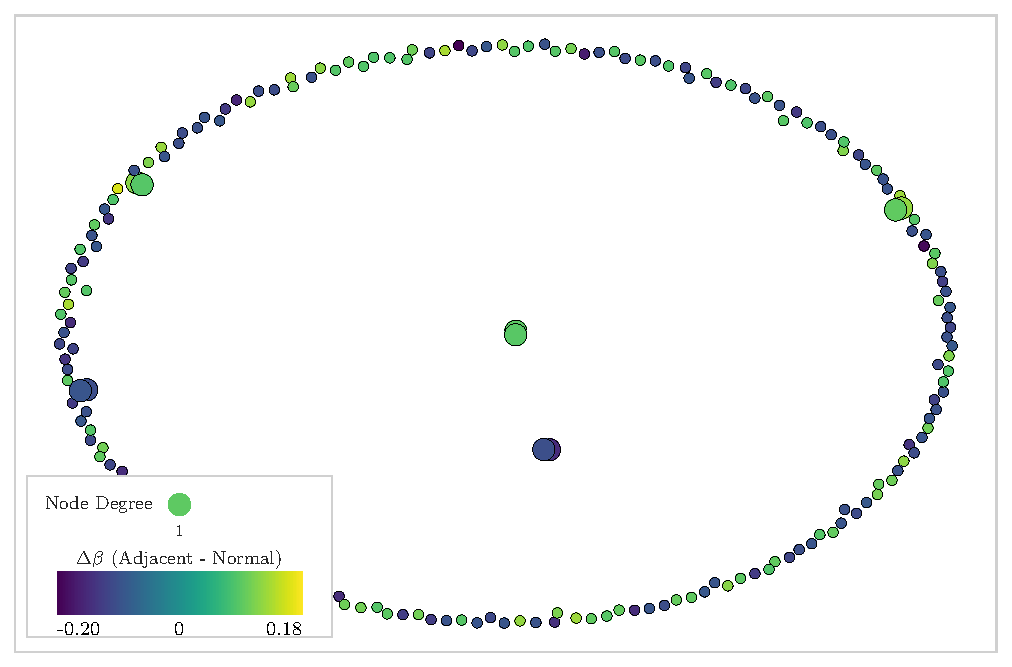
\includegraphics[width=\linewidth]{images/cap3/GSE69914_22_dnb_network_adjacent_minus_normal.pdf}
        \caption{DNB-like network: Adjacent vs Normal.}
        \label{fig:gse69914_dnb_adjacent_normal}
    \end{subfigure}
    \caption{Dynamic-network proxy visualizations in GSE69914.}
    \label{fig:gse69914_dnb_combined}
\end{figure}

Although this analysis does not follow the full mathematical formalism of Dynamic Network Biomarkers (DNBs), the degree-based and network-level (Figure~\ref{fig:gse69914_dnb_combined}) provide a qualitative view of how methylation perturbations may organize at the network level.
DNB theory, originally formulated for gene-expression and regulatory networks, predicts that near a critical transition a subset of components displays increased internal fluctuations and coordinated behaviour \cite{chen2012dnb, west2018entropy, liu2022lne}.
Here, this conceptual framework is adapted to CpG-level methylation patterns by examining the structure of CpG–gene degree distributions and the organization of $\Delta\beta$-driven network layouts. This approach enables the exploration of whether tumour-associated instability manifests as locally coordinated methylation shifts at the network level, even without implementing the complete DNB pipeline.

The degree–rank plot (Figure~\ref{fig:gse69914_dnb_degree}) displays a heavy-tailed distribution of CpG counts per gene, consistent with the heterogeneous hub–periphery structure typically observed in biological systems.
In the Tumor~vs~Normal comparison (Figure~\ref{fig:gse69914_dnb_tumor_normal}), a compact nucleus of nodes with moderately high degree is observed, accompanied by larger $\Delta\beta$ deviations.
This pattern is consistent with a more perturbed and locally coordinated subset of CpG/gene units in tumor tissue, qualitatively compatible with increased network instability.
In contrast, the Adjacent~vs~Normal network (Figure~\ref{fig:gse69914_dnb_adjacent_normal}) does not exhibit a comparable hub-like concentration and shows smaller, more diffuse deviations, suggesting that the adjacent tissue reflects only early or weakly organized perturbations.

Although these observations do not satisfy the full mathematical criteria for identifying a DNB module, they are conceptually consistent with the interpretation that tumor tissue occupies a more unstable network regime, whereas adjacent tissue remains closer to a stable (pre-transition) configuration.




% ============================================
% Summary
% ============================================
\paragraph{Overall interpretation}

The exploratory analysis of GSE69914 reveals a consistent but overall subtle separation between the three tissue states. Normal and Adjacent samples exhibit highly similar global methylation profiles, variance distributions, correlation structure, and low-dimensional embeddings, indicating that large-scale methylome organisation remains largely conserved in Adjacent tissue. Across these global summaries, the two groups are so intermixed that no clear or marked distinction emerges between Normal and Adjacent samples when using whole-methylome descriptors. Tumor samples display the expected increase in heterogeneity and a shift toward hypomethylation; however, these differences remain modest at the whole-methylome level and do not produce clear separation in unsupervised embeddings.

Locus-specific analyses, however, highlight focused patterns of disruption. Outlier CpGs exhibit both hyper- and hypomethylation events, and $\Delta\beta$ distributions reveal a distinct hypomethylation bias in Tumor samples together with a milder but detectable shift in Adjacent tissue. Dynamic-network proxies further indicate a more compact and perturbed core in Tumor samples, whereas Adjacent tissue appears more diffuse and weakly structured.

Overall, GSE69914 constitutes a technically clean dataset with well-structured methylation patterns and biologically interpretable deviations. The results indicate that tumour-related alterations are primarily localized at specific CpG loci rather than reflected in global methylome reorganization. Within this framework, the Adjacent tissue exhibits subtle yet measurable deviations from the Normal baseline, consistent with previously described field-effect patterns in breast cancer epigenomics.

% ============================================
% 2.2 GSE225845
% ============================================
\subsection{Dataset GSE225845}
\label{subsec:gse225845}

\begin{table}[t]
\centering
\caption{Overview of the GSE225845 dataset after initial cohort curation.}
\label{tab:gse225845_overview}
\scriptsize
\begin{tabular}{c c c c c}
\toprule
\textbf{CpGs} &
\textbf{Samples} &
\textbf{Normal} &
\textbf{Adjacent} &
\textbf{Tumor} \\
\midrule
750{,}426 &
477 &
113 &
140 &
224 \\
\bottomrule
\end{tabular}
\end{table}

\paragraph{Dataset overview}
\label{par:gse225845_overview}

GSE225845 is a breast tissue DNA methylation cohort profiled using the Illumina Infinium MethylationEPIC BeadChip (850K), providing genome-wide coverage of more than $8.5\times10^5$ CpG loci. The dataset is part of the NCI-Maryland Breast Cancer Cohort and includes samples spanning the Normal--Adjacent--Tumor spectrum that motivates the biological framework of this thesis.

An overview of the sample composition and CpG coverage after cohort harmonization is reported in Table~\ref{tab:gse225845_overview}, including the distribution across tissue classes.

The dataset further provides detailed demographic and clinical metadata (e.g., age at surgery, race, sex, and tissue descriptors), enabling controlled downstream analyses when required.


% ============================================
% Beta distributions
% ============================================
\paragraph{Global methylation distributions}
\label{par:gse225845_global_meth}

The group-wise mean $\beta$-value densities (Figure~\ref{fig:gse225845_group_mean_density})
display the expected bimodal configuration of EPIC arrays.
As observed in GSE69914, the three tissue groups show a high degree of overlap
across the entire $\beta$ range.

Normal and Adjacent samples exhibit nearly indistinguishable density profiles.
Tumor samples present only minimal deviations, characterised by a slight increase
in density at low $\beta$ values and a marginal attenuation of the high-$\beta$ peak.
At the whole-methylome level, no marked global redistribution of methylation levels
is evident.
\begin{figure}[t]
    \centering
    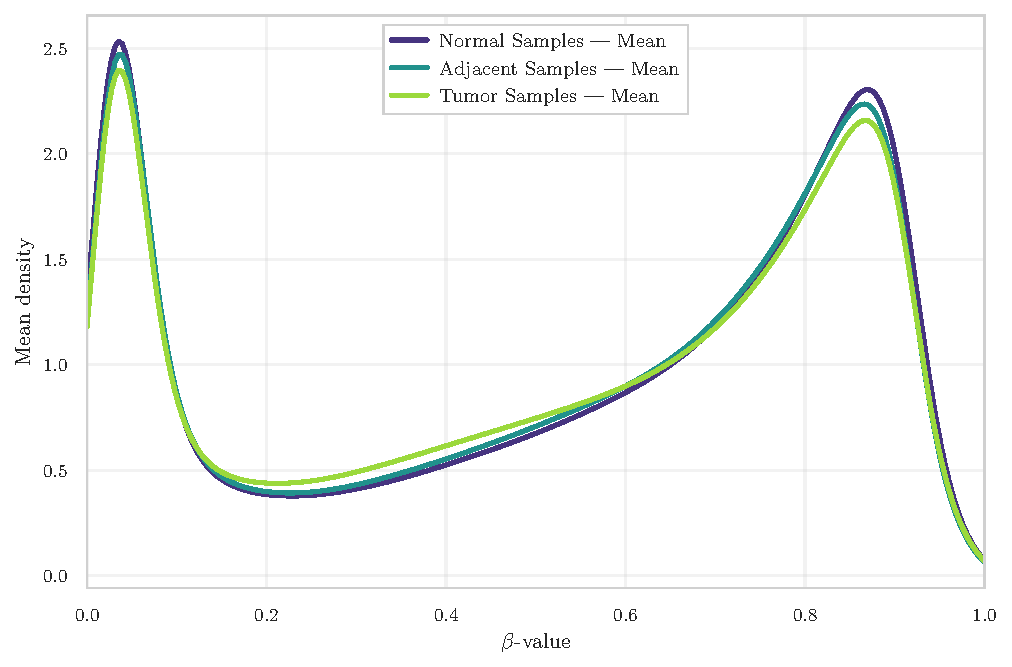
\includegraphics[width=0.5\linewidth]{images/cap3/GSE225845_04_beta_density_group_mean.pdf}
    \caption{Group-wise mean $\beta$-value density in GSE225845.}
    \label{fig:gse225845_group_mean_density}
\end{figure}




% ============================================
% Outlier burden
% ============================================
\paragraph{CpG-level instability and recurrent outliers}
\label{par:gse225845_outliers}

The heatmap of the top outlier CpG loci (Figure~\ref{fig:gse225845_outliers_heatmap})
indicates that instability within this subset is predominantly directional.
Recurrent outlier events are largely associated with very low $\beta$ values,
consistent with focal hypomethylation affecting a restricted set of CpG sites.
The perturbation pattern therefore appears concentrated rather than diffuse,
suggesting localized instability rather than a genome-wide redistribution.

The corresponding $\Delta\beta$ distributions comparing Tumor and Adjacent tissues
against Normal (Figure~\ref{fig:gse225845_outliers_deltabeta})
are sharply centered around zero, indicating that most loci remain stable.
However, both comparisons exhibit a heavier negative tail relative to the positive side.
Tumor samples display the most extended negative tail, consistent with stronger
hypomethylation shifts, whereas Adjacent tissue shows a milder but still detectable
asymmetry toward $\Delta\beta < 0$.

\begin{figure}[t]
    \centering
    \begin{subfigure}[t]{0.48\linewidth}
        \centering
        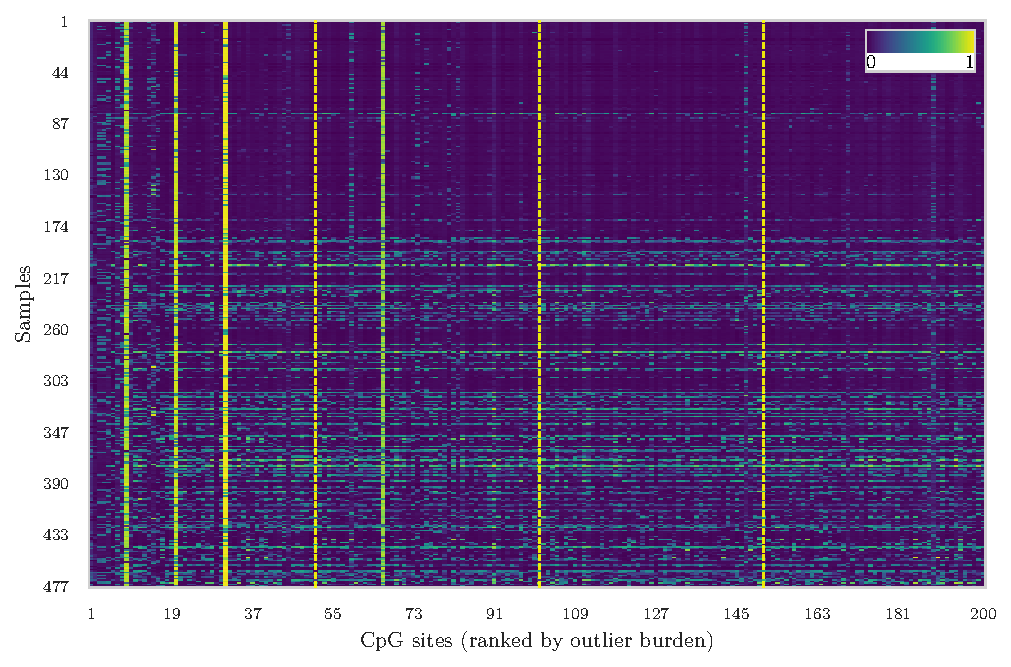
\includegraphics[width=\linewidth]{images/cap3/GSE225845_11_heatmap_top_outlier_cpgs_numbered.pdf}
        \caption{Top outlier CpG loci.}
        \label{fig:gse225845_outliers_heatmap}
    \end{subfigure}
    \hfill
    \begin{subfigure}[t]{0.48\linewidth}
        \centering
        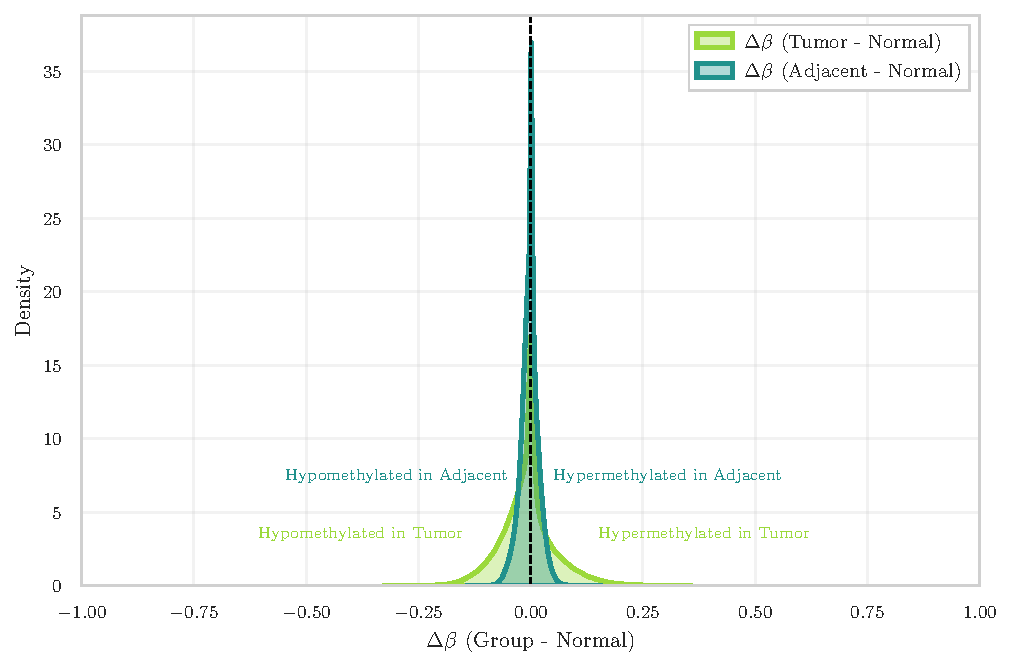
\includegraphics[width=\linewidth]{images/cap3/GSE225845_12_delta_beta_overlaid.pdf}
        \caption{$\Delta\beta$ distributions (Tumor/Adjacent $-$ Normal).}
        \label{fig:gse225845_outliers_deltabeta}
    \end{subfigure}
    \caption{Heatmap of the top outlier CpGs (left) and corresponding $\Delta\beta$ distributions (right), illustrating CpG-level instability in GSE225845.}
    \label{fig:gse225845_outliers_combined}
\end{figure}



% ============================================
% Variance, correlation, moments
% ============================================
\paragraph{Variance and correlation structure}
\label{par:gse225845_variance_corr}

The CpG-wise variance distributions (Figure~\ref{fig:gse225845_var_corr_variance})
indicate clear differences in variability across tissue groups.
Normal samples exhibit highly concentrated variance values near zero,
whereas Tumor samples display a substantially longer right tail,
reflecting an increased proportion of CpG loci with elevated variability.
Adjacent samples show a broader distribution than Normal tissues,
with partial overlap with both Normal and Tumor profiles,
but without forming a strictly intermediate pattern.

The sample correlation heatmap (Figure~\ref{fig:gse225845_var_corr_correlation})
shows uniformly positive correlations across the dataset.
Most pairwise values lie within a narrow high-correlation range,
and no distinct block structures separating tissue classes are observed.
This pattern indicates preservation of global methylation structure,
with group differences emerging primarily from locus-specific variability
rather than from large-scale shifts in overall methylome organization.

\begin{figure}[t]
    \centering
    \begin{subfigure}[t]{0.48\linewidth}
        \centering
        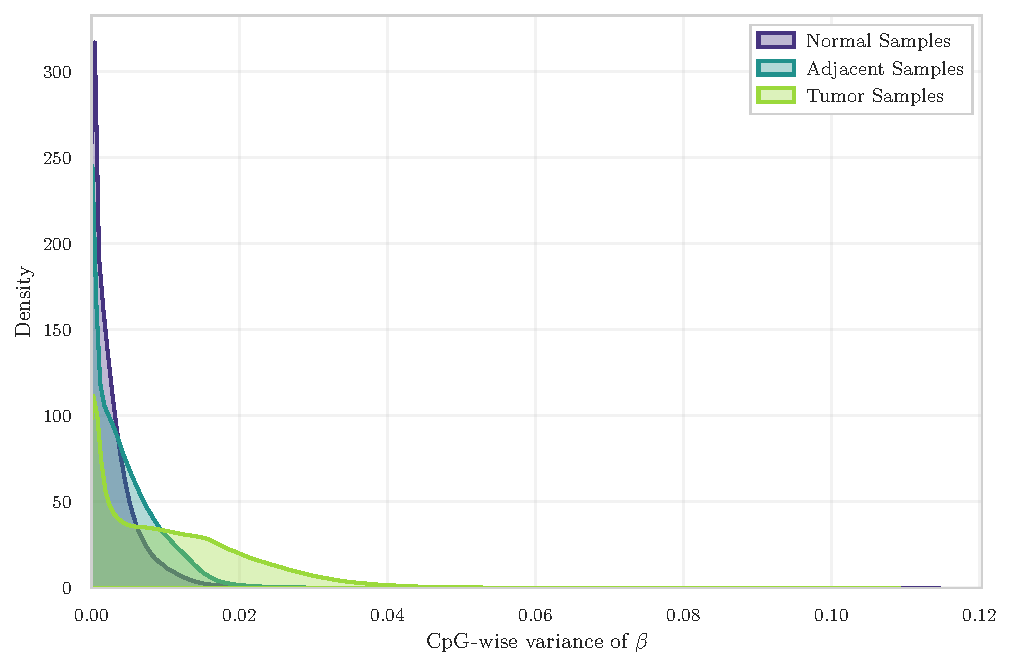
\includegraphics[width=\linewidth]{images/cap3/GSE225845_13_intragroup_variance.pdf}
        \caption{CpG-wise variance distributions.}
        \label{fig:gse225845_var_corr_variance}
    \end{subfigure}
    \hfill
    \begin{subfigure}[t]{0.48\linewidth}
        \centering
        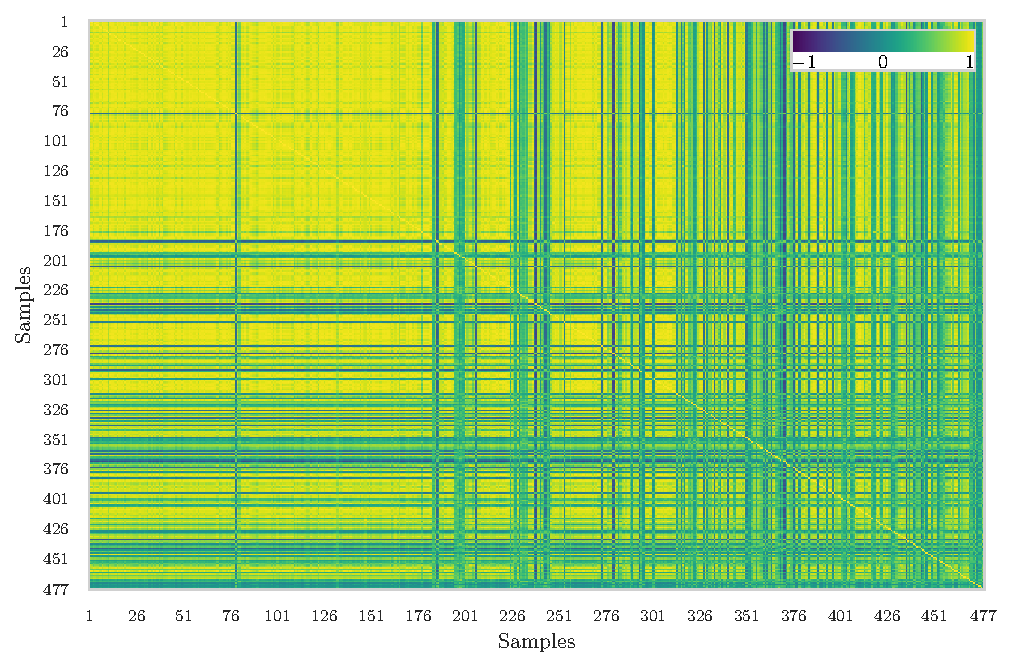
\includegraphics[width=\linewidth]{images/cap3/GSE225845_14_sample_correlation_heatmap.pdf}
        \caption{Sample correlation heatmap.}
        \label{fig:gse225845_var_corr_correlation}
    \end{subfigure}
    \caption{Variance and correlation structure across Normal, Adjacent, and Tumor samples in GSE225845.}
    \label{fig:gse225845_var_corr}
\end{figure}



% ============================================
% DR: PCA, tSNE, UMAP
% ============================================
\paragraph{Low-dimensional embeddings}
\label{par:gse225845_embeddings}

Dimensionality reduction was applied using PCA, t-SNE, and UMAP to visualise
global similarities among samples (Figure~\ref{fig:gse225845_embeddings_combined}).

In PCA space, the three tissue groups largely overlap.
Tumor samples show a slightly broader dispersion, particularly along the
second principal component, but no clear linear separation is observed.

Nonlinear embeddings reveal additional structure.
In t-SNE space, Tumor samples occupy a more extended region and appear more
dispersed, whereas Normal and Adjacent samples remain partially intermixed.
Several Tumor samples are positioned at the periphery of the embedding,
consistent with increased heterogeneity.

The UMAP projection exhibits a similar configuration.
Tumor samples span a wider area and extend toward higher values of the
second UMAP axis, while Normal and Adjacent samples form relatively
compact yet overlapping regions. Trustworthiness scores range from 0.881 to 0.939 across embeddings,
indicating good preservation of local neighbourhood structure,
particularly in the nonlinear projections. Despite differences in spread, none of the methods yields sharply
separated or isolated clusters.

\begin{figure}[t]
    \centering
    \begin{subfigure}[t]{0.32\linewidth}
        \centering
        
\includegraphics[width=\linewidth]{images/cap3/GSE225845_16_pca.pdf}
        \caption{PCA \\$\text{trustworthiness}=0.881$.}
        \label{fig:pca_gse225845}
    \end{subfigure}
    \hfill
    \begin{subfigure}[t]{0.32\linewidth}
        \centering
        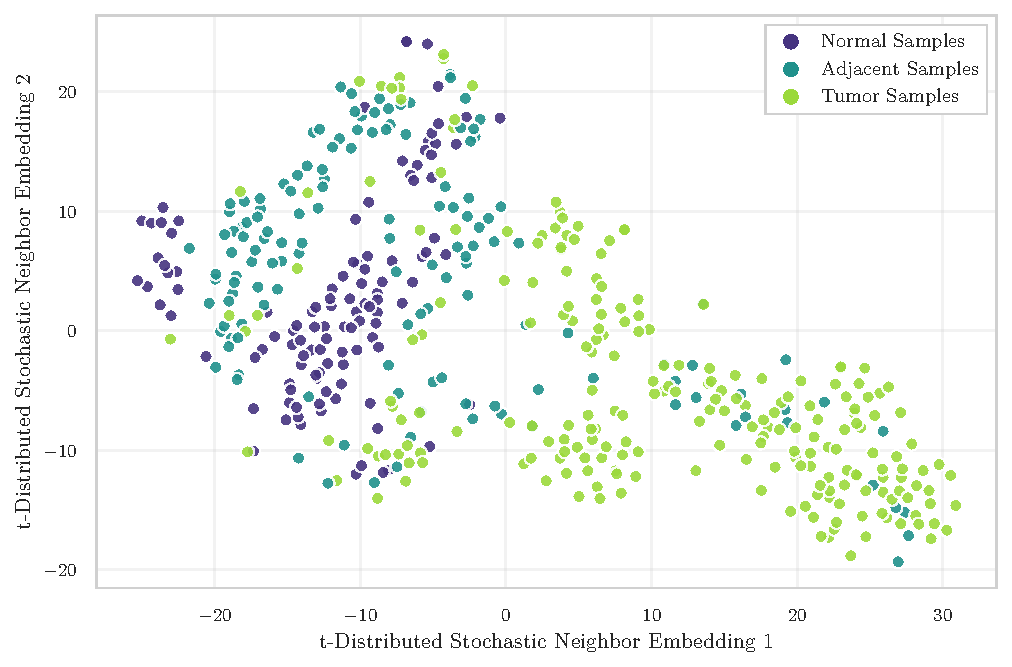
\includegraphics[width=\linewidth]{images/cap3/GSE225845_17_tsne.pdf}
        \caption{t-SNE \\$\text{trustworthiness}=0.939$.}
        \label{fig:tsne_gse225845}
    \end{subfigure}
    \hfill
    \begin{subfigure}[t]{0.32\linewidth}
        \centering
        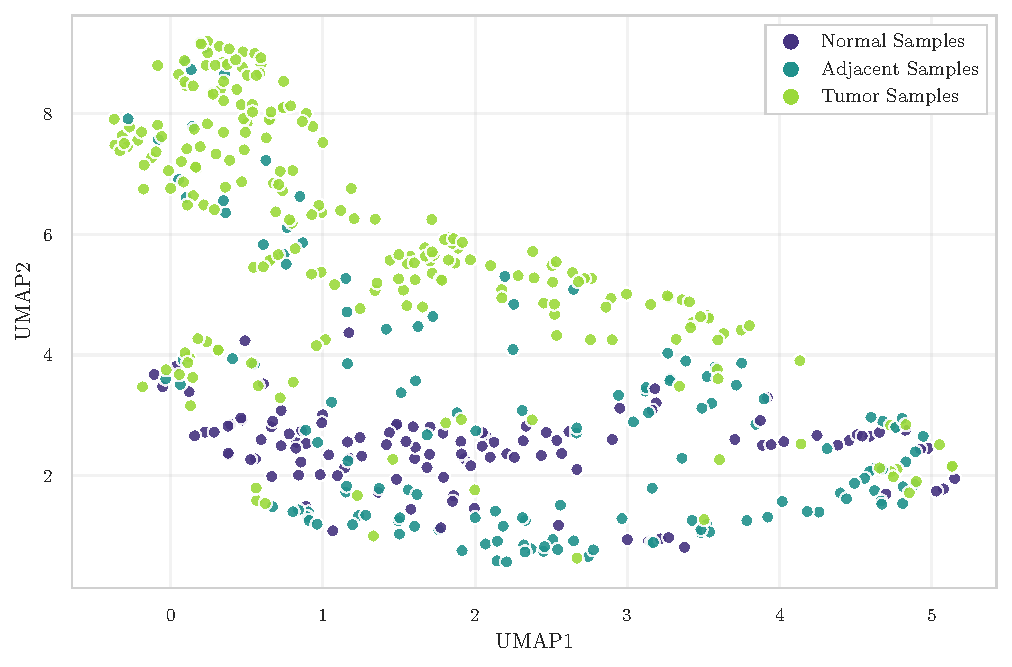
\includegraphics[width=\linewidth]{images/cap3/GSE225845_18_umap.pdf}
        \caption{UMAP \\$\text{trustworthiness}=0.894$.}
        \label{fig:umap_gse225845}
    \end{subfigure}
    \caption{Low-dimensional embeddings samples in GSE225845.}
    \label{fig:gse225845_embeddings_combined}
\end{figure}

% ============================================
% Manifest coverage
% ============================================
\paragraph{Genome annotation coverage}
\label{par:gse225845_manifest}

Consistent with the architecture of the EPIC platform, the genomic
distribution of annotated CpG contexts is markedly unbalanced.
The largest fraction of probes maps to open-sea or non-island regions,
which constitute the dominant category.
CpG islands represent the second most abundant class,
followed by north and south shores in comparable proportions,
whereas north and south shelves account for the smallest fractions.

This annotation profile aligns with the expected genomic composition of
the EPIC array and supports correct manifest integration.

% ============================================
% Dynamic network proxies
% ============================================
\paragraph{Dynamic-network proxies}
\label{par:gse225845_dnb_proxies}

The degree–rank distribution (Figure~\ref{fig:gse225845_dnb_degree})
exhibits a heavy-tailed profile, with a limited number of genes
associated with many CpGs and a long tail of low-degree nodes.
Such right-skewed degree structures are characteristic of
heterogeneous biological networks \cite{Wang2022NetworkBiology}.

In the Tumor~vs~Normal layout (Figure~\ref{fig:gse225845_dnb_tumor_normal}),
nodes aggregate into a dense and highly compact central cluster,
with only a small number of isolated peripheral points.
This geometry indicates that the largest Tumor–Normal
$\Delta\beta$ deviations are concentrated within a cohesive
subset of CpG–gene units rather than broadly distributed
across the network.

In contrast, the Adjacent~vs~Normal layout
(Figure~\ref{fig:gse225845_dnb_adjacent_normal})
displays a markedly different configuration.
While a few small central aggregates are visible,
most nodes are arranged along a wide annular structure,
forming a pronounced ring-like embedding.
This organisation reflects weaker and more spatially dispersed
deviations, without the central concentration observed
in the Tumor comparison.

Altogether, the proxy visualisations indicate that
Tumor–Normal contrasts generate a compact and locally
coherent network signal, whereas Adjacent–Normal
differences remain diffuse and geometrically fragmented.


\begin{figure}[t]
    \centering
    \begin{subfigure}[t]{0.32\linewidth}
        \centering
        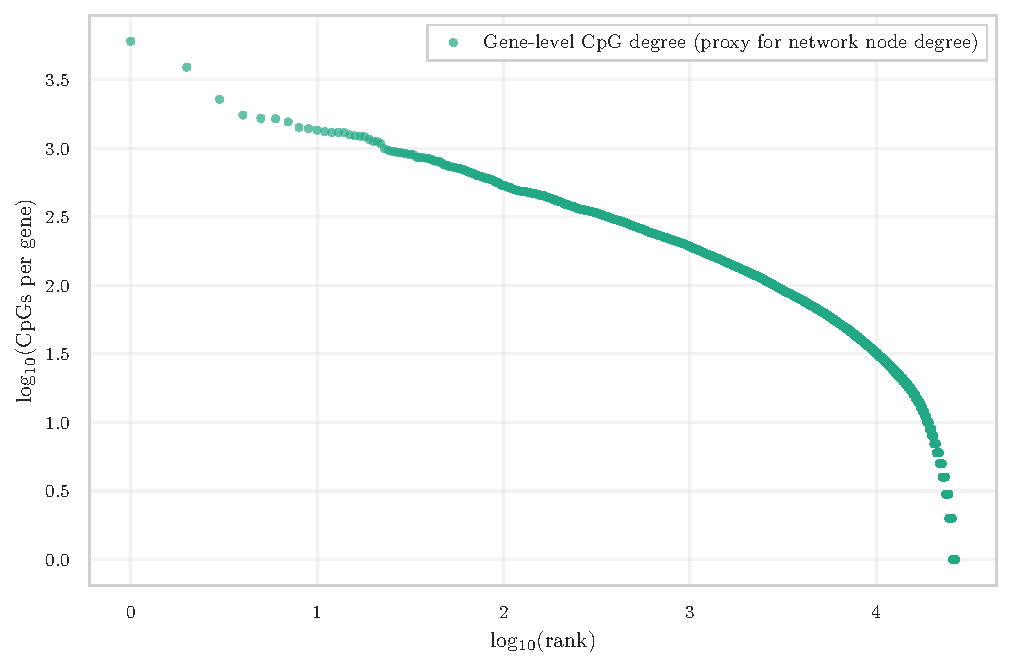
\includegraphics[width=\linewidth]{images/cap3/GSE225845_20_dynamic_network_degree_proxy.pdf}
        \caption{Gene-level CpG degree distribution.}
        \label{fig:gse225845_dnb_degree}
    \end{subfigure}
    \hfill
    \begin{subfigure}[t]{0.32\linewidth}
        \centering
        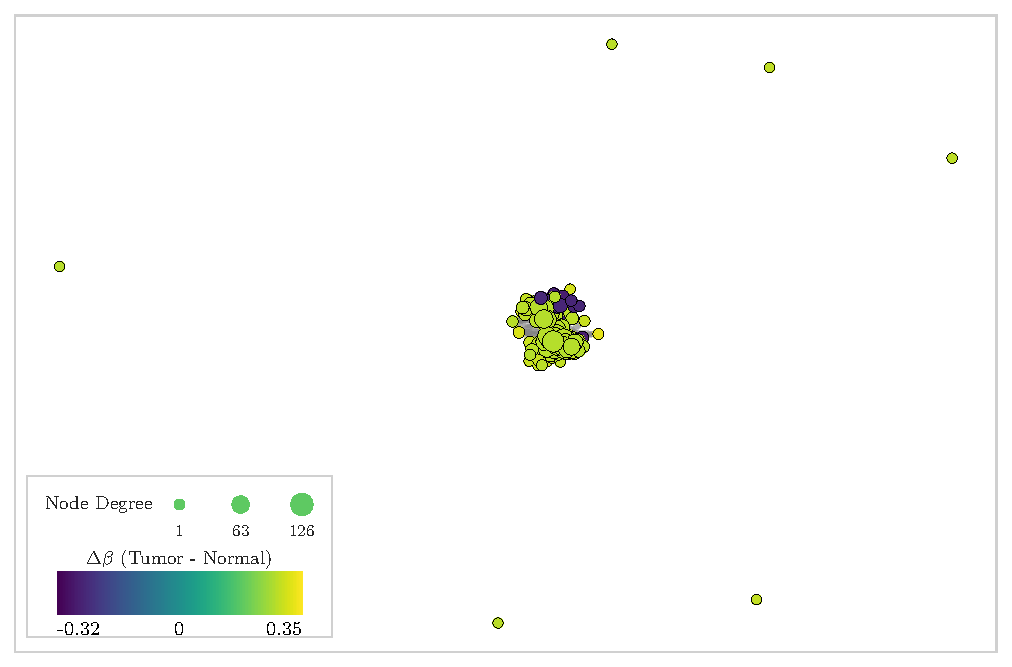
\includegraphics[width=\linewidth]{images/cap3/GSE225845_21_dnb_network_tumor_minus_normal.pdf}
        \caption{DNB-like network: Tumor vs Normal.}
        \label{fig:gse225845_dnb_tumor_normal}
    \end{subfigure}
    \hfill
    \begin{subfigure}[t]{0.32\linewidth}
        \centering
        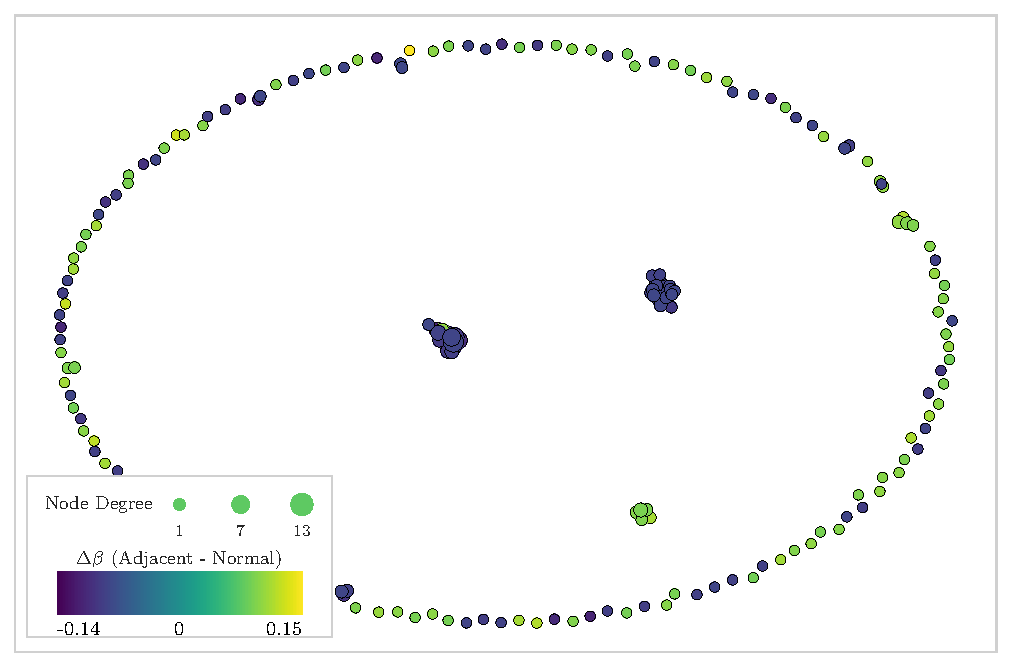
\includegraphics[width=\linewidth]{images/cap3/GSE225845_22_dnb_network_adjacent_minus_normal.pdf}
        \caption{DNB-like network: Adjacent vs Normal.}
        \label{fig:gse225845_dnb_adjacent_normal}
    \end{subfigure}
    \caption{Dynamic-network proxy visualizations in GSE225845.}
    \label{fig:gse225845_dnb_combined}
\end{figure}




% ============================================
% Summary
% ============================================
\paragraph{Overall interpretation}

The exploratory analysis of GSE225845 indicates that, at the whole-methylome level,
the three tissue states share highly similar global methylation profiles.
Group-wise mean $\beta$-value densities are nearly superimposed,
and both correlation structure and linear embeddings show substantial overlap.
These observations indicate preservation of large-scale methylome organisation
across Normal, Adjacent, and Tumor tissues, without evidence of pronounced
genome-wide redistribution of methylation levels.

Locus-focused analyses reveal more structured differences.
Among the 200 CpGs with the highest outlier burden,
instability is predominantly directional and characterised by focal hypomethylation.
Variance distributions further show increased dispersion in Tumor samples,
while Adjacent tissues exhibit broader variability than Normal
without forming a strictly intermediate pattern.

Nonlinear embeddings (t-SNE and UMAP) emphasise differences in spatial dispersion
rather than discrete cluster separation.
Normal and Adjacent samples occupy relatively compact regions,
whereas Tumor samples extend over a wider area,
reflecting increased heterogeneity.
Dynamic-network proxies show that Tumor–Normal contrasts
generate a dense central cluster of perturbed CpG–gene units,
while Adjacent–Normal differences are distributed along a broader,
ring-like structure without strong central concentration.

Despite the larger sample size of this cohort,
which provides stable estimates of global methylation structure,
the separation between Normal and Adjacent tissues remains modest.
Differences between these two groups are therefore primarily focal
and do not manifest as large-scale structural shifts.

Overall, GSE225845 represents a globally homogeneous dataset
in which tissue-state differences become apparent only when examined
through locus-specific perturbations, variability patterns,
and small-scale network organisation.



% ============================================
% 2.3 GSE287331
% ============================================
\subsection{Dataset GSE287331}
\label{subsec:gse287331}

\begin{table}[t]
\centering
\caption{Overview of the GSE287331 dataset after initial cohort curation.}
\label{tab:gse287331_overview}
\scriptsize
\begin{tabular}{c c c c c c c}
\toprule
\textbf{CpGs} &
\textbf{Samples} &
\textbf{Normal} &
\textbf{Adjacent} &
\textbf{Tumor} &
\textbf{OQ} &
\textbf{CUB} \\
\midrule
866{,}552 &
446 &
182 &
60 &
69 &
67 &
68 \\
\bottomrule
\end{tabular}
\end{table}

\begin{figure}[t]
    \centering
    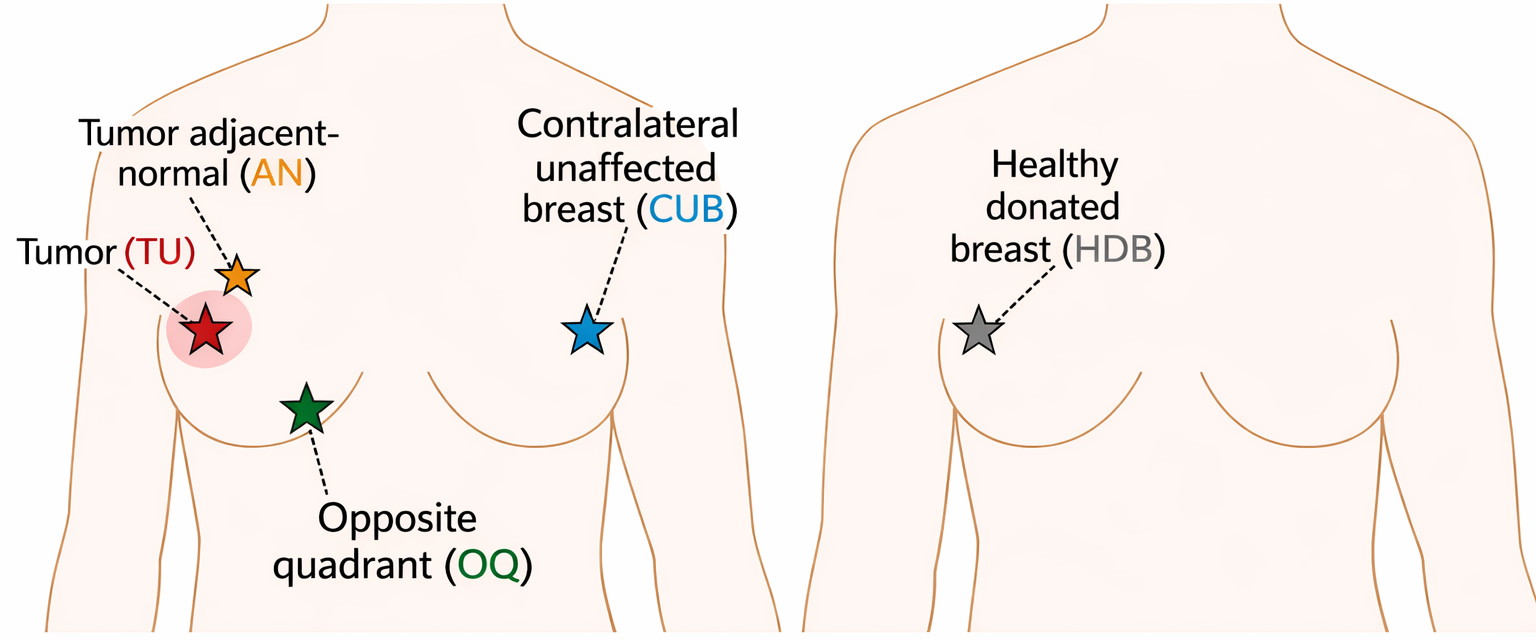
\includegraphics[width=0.7\linewidth]{images/cap3/Fig_GSE287331_Paper}
    \caption{Schematic representation of the five tissue categories collected along the tumor proximity axis (TPxA), reproduced from \cite{Lord2024GSE287331}.}
    \label{fig:gse287331_tpxa_schema}
\end{figure}

\paragraph{Dataset overview}
\label{par:gse287331_overview}

GSE287331 is a breast tissue DNA methylation cohort profiled using the
Illumina Infinium MethylationEPIC v1.0 BeadChip.
The dataset
is organised along a tumor proximity axis (TPxA) spanning multiple
anatomical and pathological contexts.

Five tissue categories are represented:
healthy donated breast (HDB), contralateral unaffected breast (CUB),
ipsilateral opposite quadrant (OQ), adjacent normal tissue (AN),
and tumor (TU). An overview of the full cohort composition is
reported in Table~\ref{tab:gse287331_overview}.

For cross-dataset consistency, only three biologically aligned classes
are retained for downstream analyses:
HDB (treated as Normal baseline),
AN (Adjacent),
and TU (Tumor).
OQ and CUB samples are excluded, as they represent intermediate
benign tissues along the proximity axis and are not directly
comparable with the three-class framework adopted in the other cohorts.


% ============================================
% Beta distributions
% ============================================

\paragraph{Global methylation distributions}
\label{par:gse287331_global_meth}

The group-wise mean $\beta$-value density curves
(Figure~\ref{fig:gse287331_group_mean_density})
display the expected bimodal configuration of Illumina methylation arrays.
A dominant peak is observed at high methylation levels, accompanied by a smaller peak consistent with standard EPIC
methylation profiles \cite{Maksimovic2017Workflow}.

Although the overall shapes remain comparable across tissue groups,
a clear ordering is visible at the high-$\beta$ peak.
Normal samples exhibit the highest density,
Adjacent samples show a slightly attenuated peak,
and Tumor samples present the lowest amplitude together
with a broader distribution extending toward intermediate
$\beta$ values.
This progressive reduction in the fully methylated peak
is consistent with increasing methylation variability
along the Normal–Adjacent–Tumor axis.

\begin{figure}[t]
    \centering
    
\includegraphics[width=0.5\linewidth]{images/cap3/GSE287331_04_beta_density_group_mean.pdf}
    \caption{Group-wise mean $\beta$-value density in GSE287331.}
    \label{fig:gse287331_group_mean_density}
\end{figure}



% ============================================
% Outlier burden
% ============================================
\paragraph{CpG-level instability and recurrent outliers}
\label{par:gse287331_outliers}

The heatmap of the top outlier CpG loci
(Figure~\ref{fig:gse287331_outliers_heatmap})
shows that epigenetic instability is not uniformly distributed.
Alterations concentrate at specific CpG sites and within specific
samples, forming vertical and horizontal bands rather than a
diffuse genome-wide pattern.
Both directions of deviation are observed, with focal
hypermethylation and focal hypomethylation present within the selected loci
\cite{ehrlich2002}.

The corresponding $\Delta\beta$ distributions
(Figure~\ref{fig:gse287331_outliers_deltabeta})
highlight distinct profiles for the two contrasts.
The Tumor–Normal curve is broader and displays a higher density
of small negative shifts, indicating widespread but moderate
hypomethylation in Tumor samples.
In contrast, the Adjacent–Normal distribution is more sharply
centered around zero but exhibits a comparatively more pronounced
negative tail, reflecting fewer yet larger hypomethylated deviations.
Overall, hypomethylation represents the dominant direction of
change in both comparisons.

\begin{figure}[t]
    \centering
    \begin{subfigure}[t]{0.48\linewidth}
        \centering
        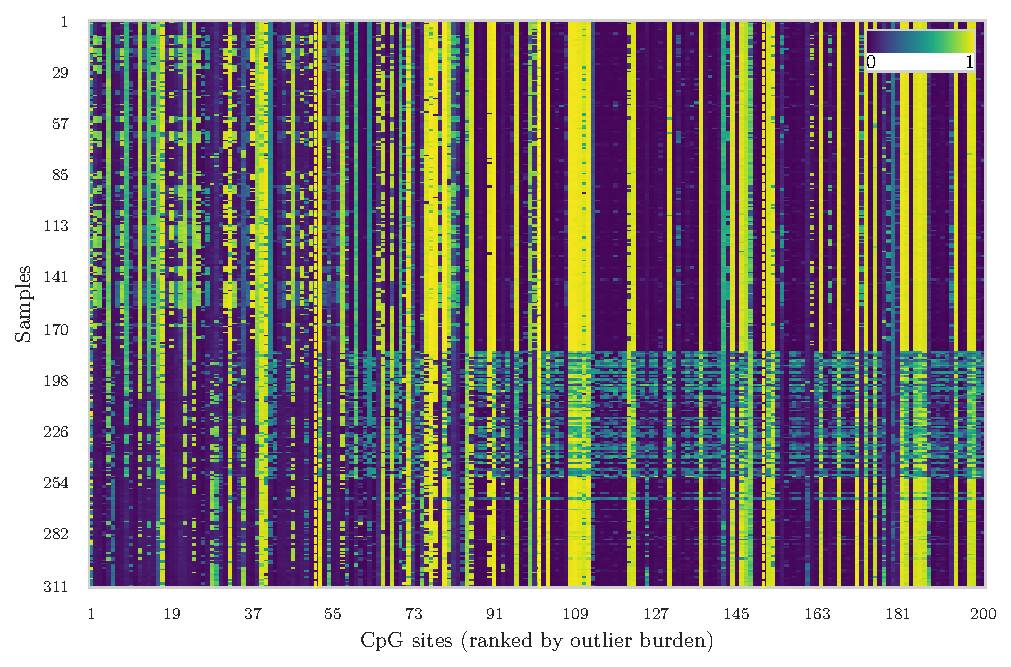
\includegraphics[width=\linewidth]{images/cap3/GSE287331_11_heatmap_top_outlier_cpgs_numbered.pdf}
        \caption{Top outlier CpG loci.}
        \label{fig:gse287331_outliers_heatmap}
    \end{subfigure}
    \hfill
    \begin{subfigure}[t]{0.48\linewidth}
        \centering
        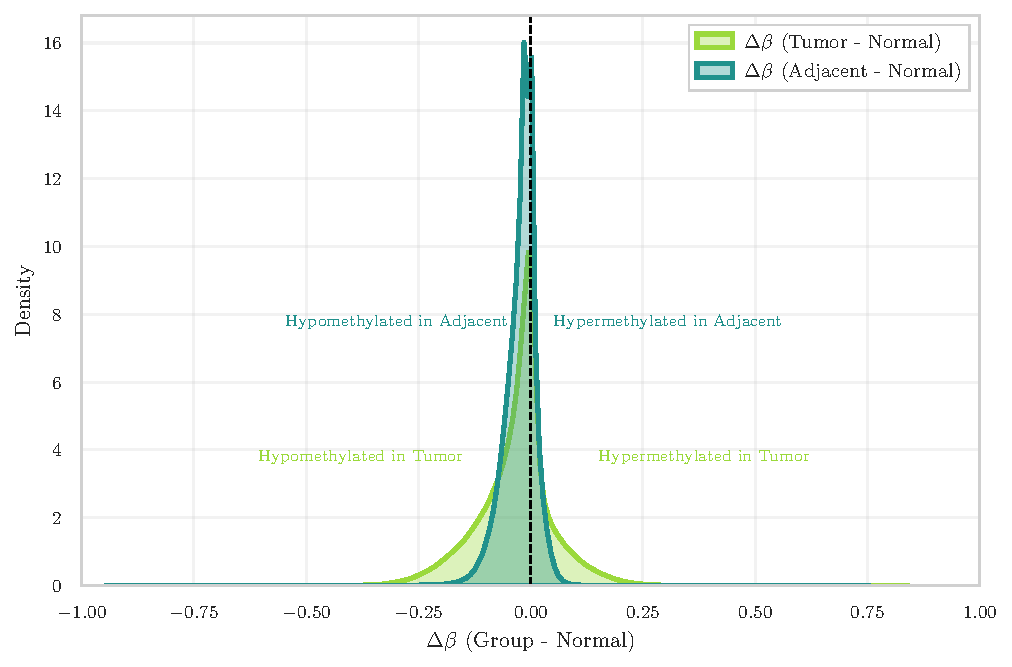
\includegraphics[width=\linewidth]{images/cap3/GSE287331_12_delta_beta_overlaid.pdf}
        \caption{$\Delta\beta$ distributions (Tumor/Adjacent $-$ Normal).}
        \label{fig:gse287331_outliers_deltabeta}
    \end{subfigure}
    \caption{Heatmap of the top outlier CpGs (left) and corresponding $\Delta\beta$ distributions (right), illustrating CpG-level instability in GSE287331.}
    \label{fig:gse287331_outliers_combined}
\end{figure}



% ============================================
% Variance, correlation, moments
% ============================================
\paragraph{Variance and correlation structure}
\label{par:gse287331_variance_corr}

The CpG-wise variance density curves
(Figure~\ref{fig:gse287331_var_corr_variance})
show that Normal and Adjacent samples are nearly superimposed,
with both groups exhibiting extremely low and tightly
concentrated variance values.
Tumor samples display a slightly broader right tail,
indicating modestly increased genome-wide variability;
however, the overall distribution remains sharply peaked
near zero.

At the level of CpG-wise variance, Adjacent tissue
remains closely aligned with the Normal baseline,
whereas Tumor samples show only a mild elevation
in variability.

A complementary perspective is provided by the
sample correlation heatmap
(Figure~\ref{fig:gse287331_var_corr_correlation}).
Correlations are uniformly high across the cohort,
consistent with the predominance of stable CpG loci
in genome-wide methylation data \cite{Teschendorff2013BMIQ}.
Although tissue labels are not overlaid on the matrix,
localized blocks of higher similarity are visible,
indicating structured relationships within subsets
of samples rather than abrupt global separation.  

\begin{figure}[t]
    \centering
    \begin{subfigure}[t]{0.48\linewidth}
        \centering
        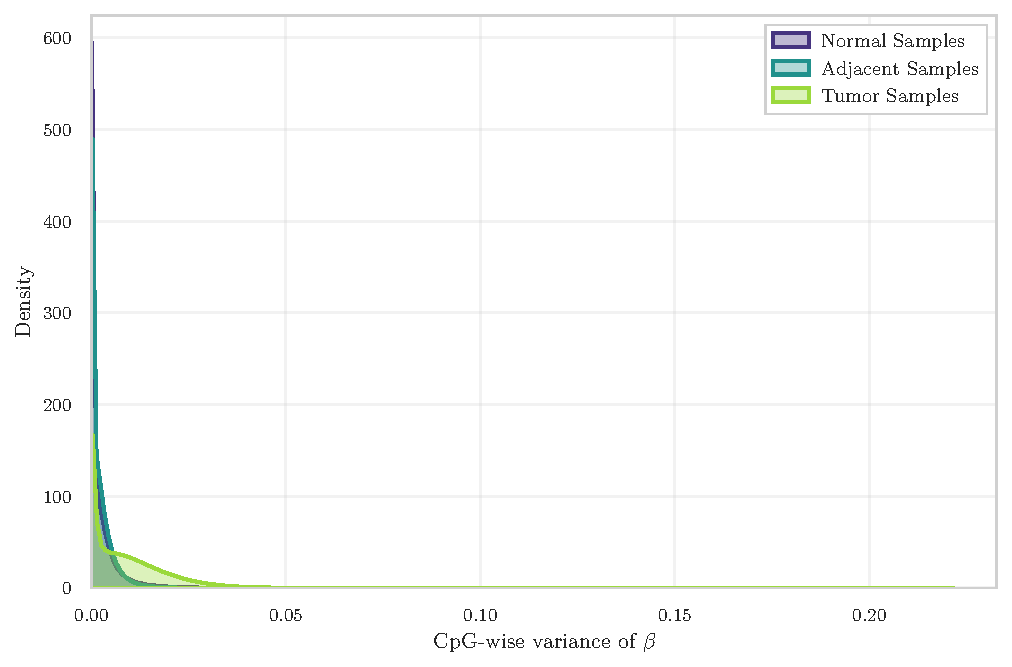
\includegraphics[width=\linewidth]{images/cap3/GSE287331_13_intragroup_variance.pdf}
        \caption{CpG-wise variance distributions.}
        \label{fig:gse287331_var_corr_variance}
    \end{subfigure}
    \hfill
    \begin{subfigure}[t]{0.48\linewidth}
        \centering
        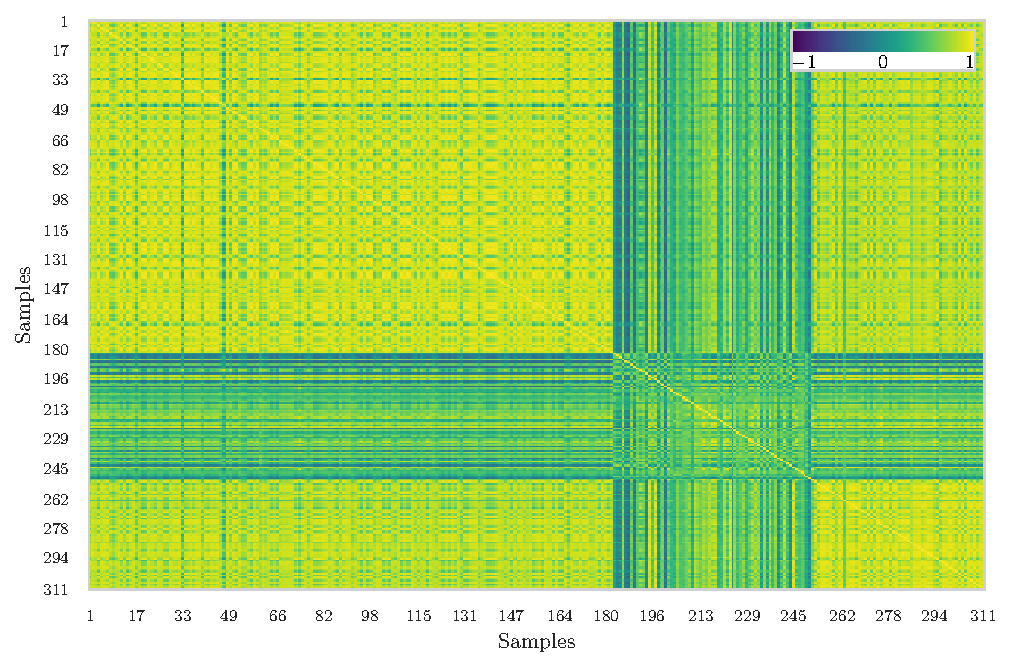
\includegraphics[width=\linewidth]{images/cap3/GSE287331_14_sample_correlation_heatmap.pdf}
        \caption{Sample correlation heatmap.}
        \label{fig:gse287331_var_corr_correlation}
    \end{subfigure}
    \caption{Variance and correlation structure across Normal, Adjacent, and Tumor samples in GSE287331.}
    \label{fig:gse287331_var_corr}
\end{figure}



% ============================================
% DR: PCA, tSNE, UMAP
% ============================================
\paragraph{Low-dimensional embeddings}
\label{par:gse287331_embeddings}

Dimensionality reduction using PCA, t-SNE, and UMAP
was applied to visualise the global organisation of methylation profiles
(Figure~\ref{fig:gse287331_embeddings_combined}).

Across all three embeddings, a consistent and well-defined structure is observed.
Normal and Adjacent samples form two clearly separated clusters.
The separation is visible in PCA space,
becomes more pronounced in t-SNE,
and appears as fully detached manifolds in the UMAP projection.

Tumor samples occupy a distinct and more dispersed region of the embedding space,
reflecting increased epigenetic heterogeneity. Trustworthiness scores are uniformly high (0.961–0.980),
indicating excellent preservation of local neighbourhood structure
in all low-dimensional projections. No substantial overlap between Tumor and the other two groups
is observed in any of the projections,
indicating strong intrinsic group structure in this cohort.
\begin{figure}[t]
    \centering
    \begin{subfigure}[t]{0.32\linewidth}
        \centering
        
\includegraphics[width=\linewidth]{images/cap3/GSE287331_16_pca.pdf}
        \caption{PCA \\$\text{trustworthiness}=0.961$.}
    \end{subfigure}
    \hfill
    \begin{subfigure}[t]{0.32\linewidth}
        \centering
        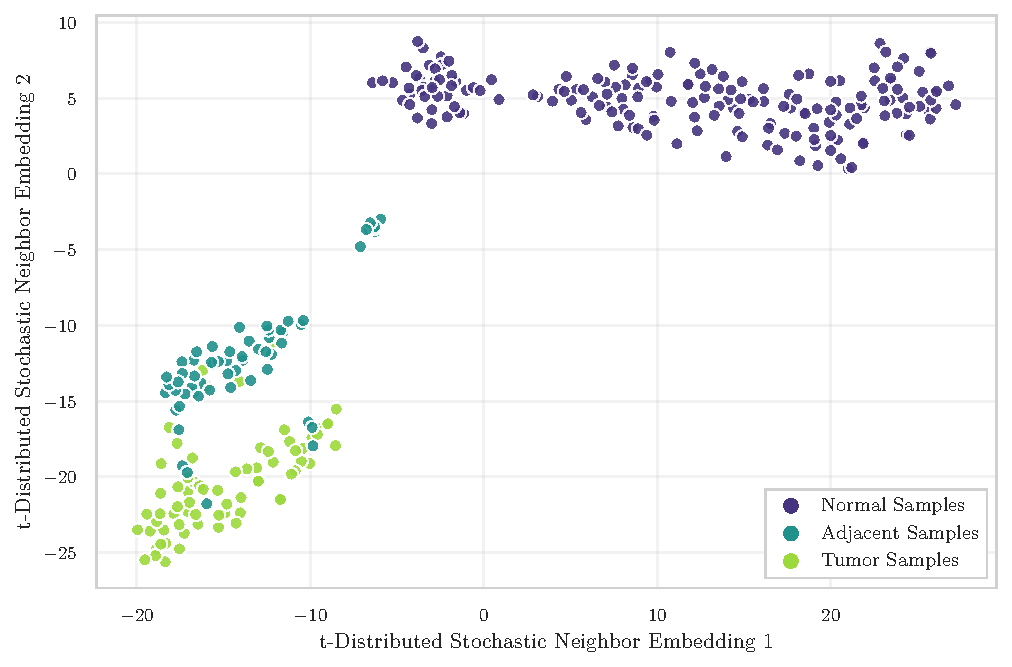
\includegraphics[width=\linewidth]{images/cap3/GSE287331_17_tsne.pdf}
        \caption{t-SNE \\$\text{trustworthiness}=0.980$.}
    \end{subfigure}
    \hfill
    \begin{subfigure}[t]{0.32\linewidth}
        \centering
        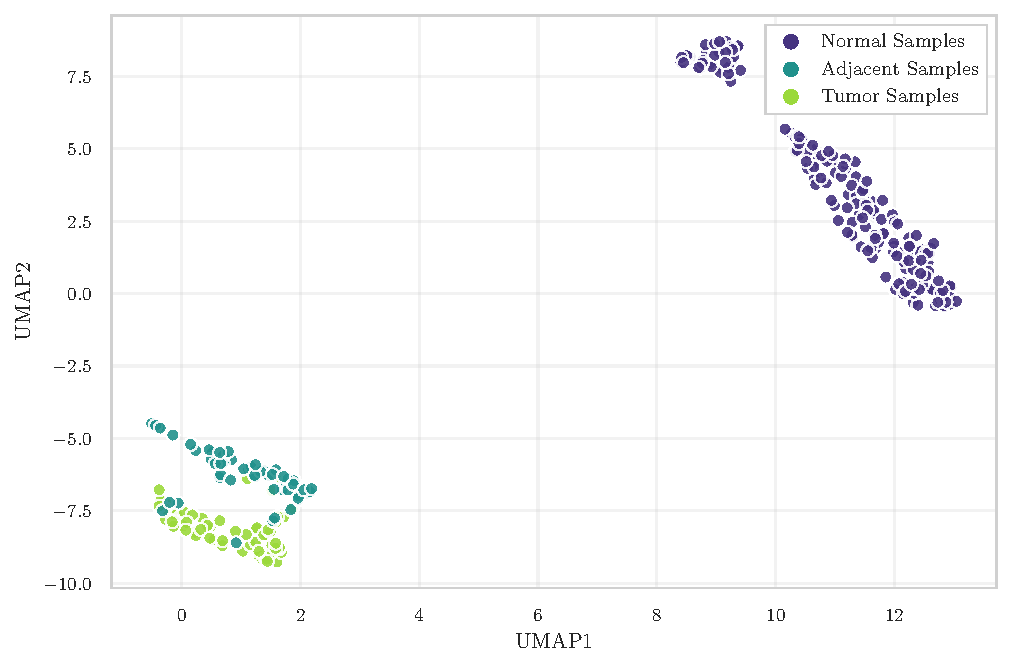
\includegraphics[width=\linewidth]{images/cap3/GSE287331_18_umap.pdf}
        \caption{UMAP \\$\text{trustworthiness}=0.973$.}
    \end{subfigure}
    \caption{Low-dimensional embeddings of GSE287331 samples.}
    \label{fig:gse287331_embeddings_combined}
\end{figure}

% ============================================
% Manifest coverage
% ============================================
\paragraph{Genome annotation coverage}
\label{par:gse287331_manifest}

The genomic distribution of annotated CpG contexts
is dominated by Open Sea regions, followed by CpG
Islands, then Shores, with Shelves representing
the smallest fractions.

This ordering is consistent with the established
architecture of EPIC arrays
\cite{zhou2017, pidsley2016}.

% ============================================
% Dynamic network proxies
% ============================================
\paragraph{Dynamic-network proxies}
\label{par:gse287331_dnb_proxies}

The degree–rank curve 
(Figure~\ref{fig:gse287331_dnb_degree}) shows a heavy-tailed distribution of CpG counts 
per gene, consistent with a hub–periphery architecture typical of biological networks.  

Both $\Delta\beta$-based network layouts — Tumor vs Normal and Adjacent vs Normal 
(Figure~\ref{fig:gse287331_dnb_tumor_normal}, 
Figure~\ref{fig:gse287331_dnb_adjacent_normal}) — share a similar overall structure:  
a dense and compact central block of nodes connected by short-range edges, 
surrounded by a ring of peripheral, weakly connected nodes.  
This geometry reflects the underlying degree distribution and indicates that most 
CpG–gene units contribute only minimally to group-level differences.

Despite this shared organisation, the Tumor vs Normal comparison exhibits a more 
pronounced central cluster with larger $\Delta\beta$ magnitudes, suggesting that a 
restricted subset of CpG–gene units undergoes locally coordinated perturbations.  
In contrast, the Adjacent vs Normal layout preserves the same global shape but 
shows weaker deviations, indicating only mild coordination of methylation changes.
\begin{figure}[t]
    \centering
    \begin{subfigure}[t]{0.32\linewidth}
        \centering
        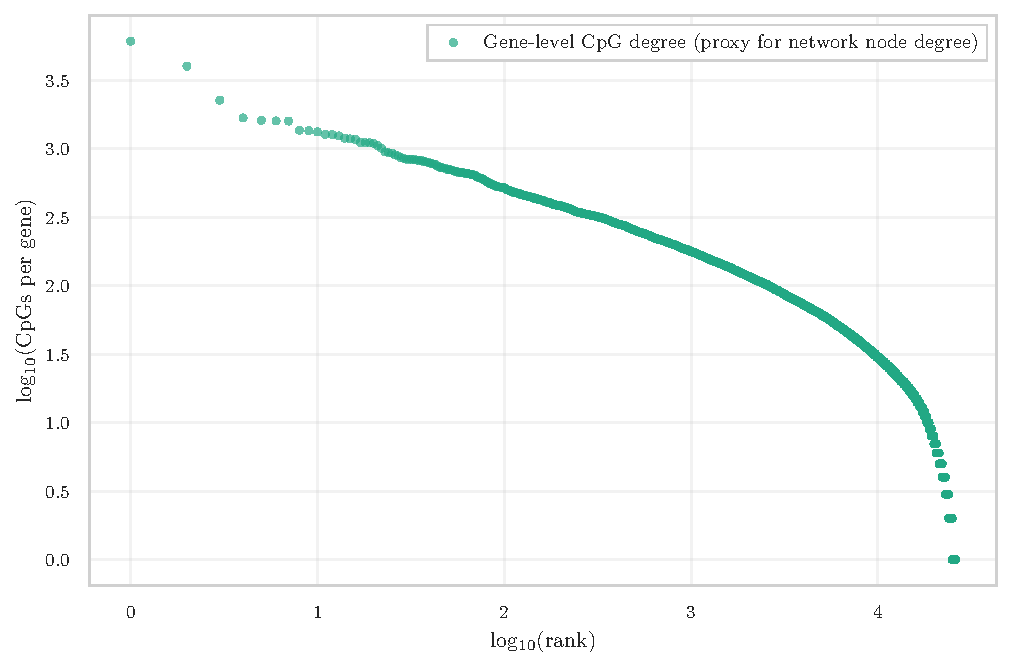
\includegraphics[width=\linewidth]{images/cap3/GSE287331_20_dynamic_network_degree_proxy.pdf}
        \caption{Gene-level CpG degree distribution.}
        \label{fig:gse287331_dnb_degree}
    \end{subfigure}
    \hfill
    \begin{subfigure}[t]{0.32\linewidth}
        \centering
        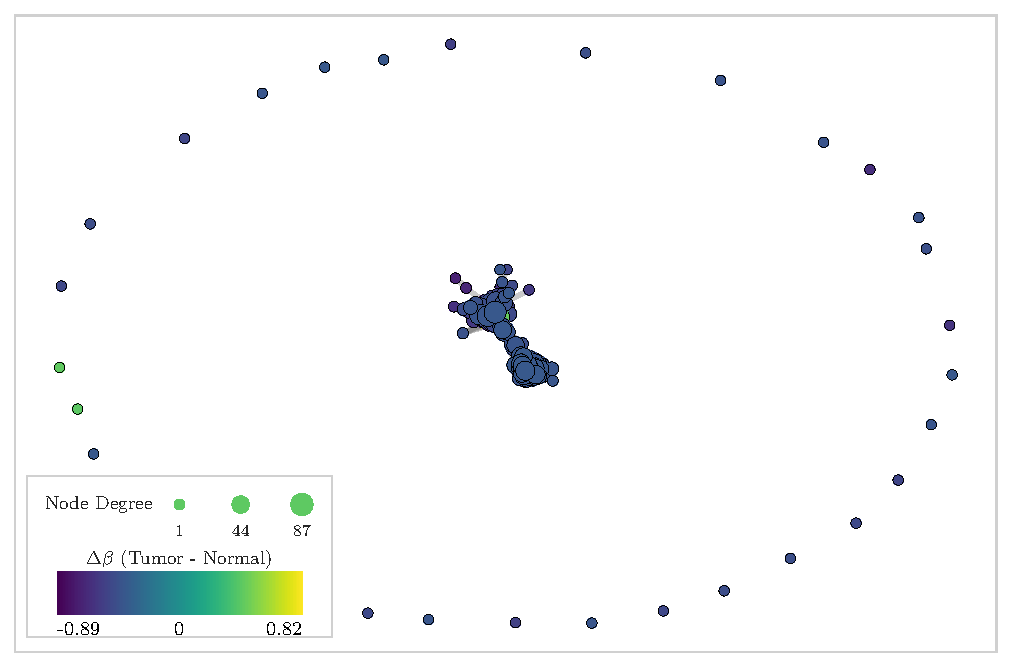
\includegraphics[width=\linewidth]{images/cap3/GSE287331_21_dnb_network_tumor_minus_normal.pdf}
        \caption{DNB-like network: Tumor vs Normal.}
        \label{fig:gse287331_dnb_tumor_normal}
    \end{subfigure}
    \hfill
    \begin{subfigure}[t]{0.32\linewidth}
        \centering
        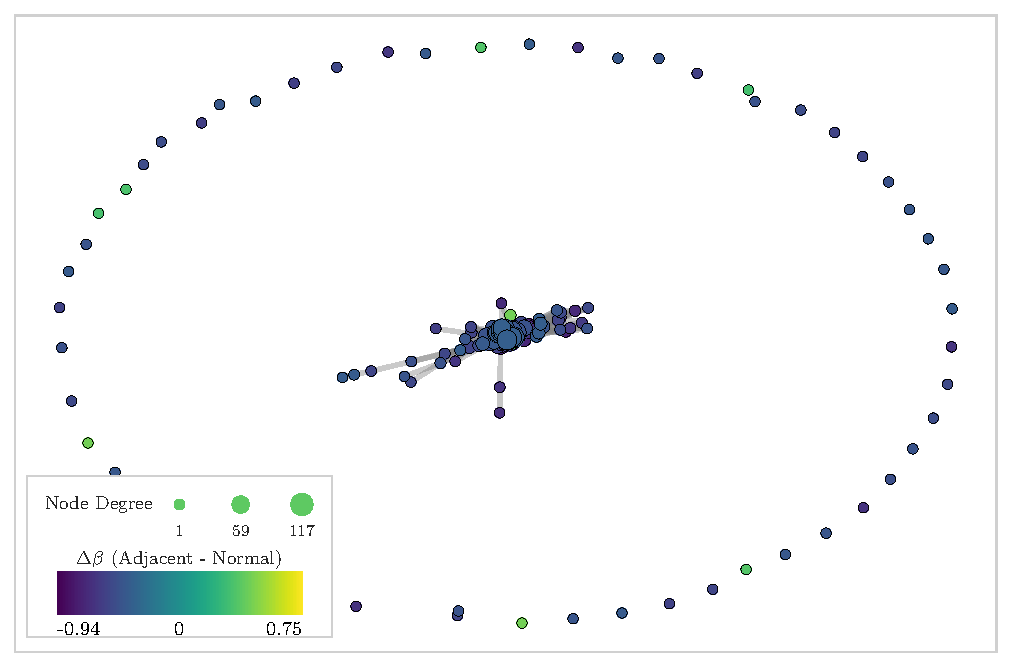
\includegraphics[width=\linewidth]{images/cap3/GSE287331_22_dnb_network_adjacent_minus_normal.pdf}
        \caption{DNB-like network: Adjacent vs Normal.}
        \label{fig:gse287331_dnb_adjacent_normal}
    \end{subfigure}
    \caption{Dynamic-network proxy visualizations for GSE287331.}
    \label{fig:gse287331_dnb_combined}
\end{figure}



% ============================================
% Summary
% ============================================
\paragraph{Overall interpretation}

The exploratory analysis of GSE287331 indicates that, at the whole-methylome level,
the three tissue states retain a broadly preserved global methylation architecture. Group-wise mean $\beta$-value densities follow the typical bimodal EPIC profile
with only a subtle gradient (Normal $>$ Adjacent $>$ Tumor),
and both CpG-wise variance distributions and sample correlation structure
show high overall similarity across tissues, with only mild variability increases in Tumor samples.

In contrast to the previous cohorts, low-dimensional embeddings reveal
a clear and consistent separation of all three groups. Normal and Adjacent samples form distinct clusters in PCA,
with the separation further strengthened in t-SNE and UMAP,
where the groups appear as detached manifolds. Tumor samples occupy a separate and more diffuse region,
reflecting increased epigenetic heterogeneity. These projections indicate that, despite similar first- and second-order
global summaries, multivariate structure in this dataset
captures strong group-level organisation.

Locus-specific analyses reveal focused disruptions. Tumor samples exhibit widespread mild hypomethylation,
whereas Adjacent tissue shows fewer but larger-magnitude deviations.
Dynamic-network proxies further indicate a compact and perturbed
central core in the Tumor comparison,
while Adjacent–Normal differences display weaker coordination,
consistent with early-stage methylation alterations.

Overall, GSE287331 emerges as a structurally coherent and biologically
informative dataset in which Normal–Adjacent–Tumor separation
is markedly more pronounced than in the other cohorts,
while global methylation architecture remains broadly conserved.


% ============================
% Inter Dataset Analysis
% ============================
\section{Inter Dataset Exploration and Comparison}
\label{sec:inter_dataset}

The objective of this section is not to merge the datasets—an approach that would be biologically and technically inappropriate due to differences in array platforms (HM450 vs.\ EPIC), preprocessing pipelines—but rather to compare their internal behaviours. Such a cross-dataset perspective enables the assessment of whether the early epigenetic alterations identified in the intra-dataset analyses are \emph{reproducible across independent cohorts}, thereby providing support for the central biological premise of this thesis: the detection of early methylation drift in histologically normal tissues and the evaluation of its potential contribution to tumour initiation.

\subsection{Analytical Framework}

Across all three datasets, the intra-dataset analyses revealed three highly consistent phenomena:

\begin{itemize}[label=--]
    \item Normal and Adjacent tissues are globally similar, with nearly superimposed $\beta$-value distributions and
    comparable CpG-wise variance profiles.
    \item Tumour samples show increased heterogeneity and a clear bias toward hypomethylation, although the magnitude
    of this shift varies across datasets.
    \item Adjacent tissues exhibit early methylation drift, detectable through $\Delta\beta$ distributions and outlier 
    profiles even when global metrics remain highly similar to Normal.
\end{itemize}

These patterns are consistent with the expected biological progression from Normal to Tumour, in which epigenetic 
deregulation emerges gradually and affects normal-appearing tissue surrounding the tumour.  
The inter-dataset analysis therefore evaluates the \textit{directional consistency} of these effects rather than aiming 
at strict quantitative comparability.

\subsection{Cross-Dataset Comparative Metric}

\begin{table}[t]
\centering
\caption{Cross-dataset comparison of Normal (N) vs Adjacent (A) contrasts using global and instability metrics.}
\label{tab:inter_summary_NA}
\scriptsize
\begin{tabular}{lcccc}
\toprule
\textbf{Dataset} &
\textbf{Mean $|\Delta\beta|$ (A--N)} &
\textbf{Var Ratio (A/N)} &
\textbf{Outlier Ratio (A/N)} &
\textbf{Silhouette (A/N)} \\
\midrule
GSE69914 &
0.009 &
0.988 &
1.353 &
0.003 \\
GSE225845 &
0.015 &
0.972 &
2.790 &
0.042 \\
GSE287331 &
0.031 &
0.930 &
13.329 &
0.344 \\
\bottomrule
\end{tabular}
\end{table}

To quantify the epigenetic deviation of Adjacent tissue from the Normal methylome across the three cohorts, a set of global and instability-oriented metrics was computed independently within each dataset for the Adjacent versus Normal contrast.

All metrics reported in Table~\ref{tab:inter_summary_NA} were computed using the complete CpG set available in each dataset, rather than the cross-platform intersection. The resulting values therefore reflect cohort-specific dimensionality and internal variance structure.

Collectively, these metrics indicate the presence of early epigenetic drift in histologically non-tumour tissue. Across cohorts, increasing mean $|\Delta\beta|$, progressive variance imbalance, elevated outlier ratios, and improved silhouette separation consistently support a directional shift from Normal to Adjacent states, in agreement with the field-defect framework described by Teschendorff et~\cite{teschendorff2016} and reinforced in other tissue contexts.

\paragraph{Mean absolute methylation difference}  

For each CpG, the absolute mean difference between Adjacent and Normal was defined as
\begin{equation}
|\Delta\beta_i| = \left| \beta^{(A)}_i - \beta^{(N)}_i \right|.
\label{eq:mean_abs_delta_beta}
\end{equation}

The cross-cohort pattern reveals progressively larger locus-specific shifts from GSE69914 to GSE225845 and GSE287331.  
Although the absolute magnitude of the effect remains modest, it is consistent in direction across cohorts.  
This monotonic increase reflects a strengthening early deviation in Adjacent tissues. Comparable locus-wise methylation drifts in histologically normal tissue have been reported in independent systems, such as colonic mucosa adjacent to adenomas~\cite{Yates2024_NormalMucosaField}, supporting the interpretation of these alterations as early manifestations of field cancerization.

\paragraph{Global variance ratio}  

For each sample $s$, the global methylation variance was computed across all CpG sites:
$
v_s = \mathrm{Var}\!\left(\beta_{s,1}, \beta_{s,2}, \ldots, \beta_{s,m}\right),
$
where $m$ denotes the number of CpGs. Group-wise mean variances were then defined as
\begin{equation}
\overline{v}^{(N)} = \frac{1}{|N|} \sum_{s \in N} v_s,
\qquad
\overline{v}^{(A)} = \frac{1}{|A|} \sum_{s \in A} v_s,
\label{eq:group_mean_variance}
\end{equation}
and the reported metric corresponds to their ratio:
\begin{equation}
\mathrm{\frac{Var(A)}{Var(N)}} = 
\frac{\overline{v}^{(A)}}{\overline{v}^{(N)}}.
\label{eq:variance_ratio}
\end{equation}

Across cohorts, this ratio remained consistently close to unity, indicating that Adjacent tissue does not exhibit diffuse genome-wide instability.  
Such behaviour suggests that early pre-neoplastic alterations are predominantly \emph{focal} rather than global, with only specific CpG sites displaying abnormal dispersion while overall variance remains largely preserved~\cite{Yates2024_NormalMucosaField}.  

This interpretation is consistent with contemporary models of early tumourigenesis, in which subtle and locally restricted perturbations accumulate prior to large-scale chromatin deregulation and overt neoplastic transformation~\cite{Zhang2024_TumorInitiationEpigenetic}.


\paragraph{Outlier burden ratio}  
For each sample, the outlier burden is defined as the number of CpG sites whose methylation 
deviates from the Normal reference distribution by more than three times the Normal 
interquartile range:
\begin{equation}
\text{outlier}_s = 
\#\left\{\, i \;:\; 
\left| \beta_{i,s} - \tilde{\beta}^{(N)}_i \right| 
> 3 \cdot IQR^{(N)}_i \,\right\},
\label{eq:outlier_burden}
\end{equation}
where $\tilde{\beta}^{(N)}_i$ and $IQR^{(N)}_i$ denote the median and interquartile range of CpG $i$ 
across Normal samples.  

The reported A/N ratio corresponds to the mean outlier burden in Adjacent tissue divided by the 
mean burden in Normal tissue. Across cohorts, this metric exhibits the most pronounced cross-dataset gradient, with progressively stronger enrichment of outlier events in Adjacent tissue.  
Such behaviour mirrors evidence that increased local methylation variability in histologically normal tissue represents a sensitive marker of early instability~\cite{Yates2024_NormalMucosaField}, and provides quantitative support for the presence of marked field effects in GSE287331.

\paragraph{Silhouette score}  

For each sample $s$, let $a(s)$ denote the mean distance from $s$ to all other samples within the same group (cohesion), and let $b(s)$ denote the smallest mean distance from $s$ to samples in the alternative group (separation).  
The silhouette coefficient for sample $s$ is defined as
\begin{equation}
\mathrm{sil}(s) =
\frac{b(s) - a(s)}{\max\{a(s),\, b(s)\}},
\label{eq:silhouette}
\end{equation}
and the reported score corresponds to the mean silhouette computed across all Normal and Adjacent samples.

Higher values indicate clearer multivariate separation between Normal and Adjacent states, whereas values near zero reflect substantial overlap. Across cohorts, the silhouette analysis reveals limited separation in GSE69914 and GSE225845, consistent with minimal global displacement in multivariate space. In contrast, GSE287331 exhibits partial separation, indicating that the epigenetic landscape of Adjacent tissue is measurably shifted relative to Normal. This behaviour aligns with mechanistic models in which epigenetic dysregulation constitutes one of the earliest events in tumour initiation~\cite{Zhang2024_TumorInitiationEpigenetic}, preceding morphological transformation.

Collectively, the set of metrics delineates a consistent Normal--Adjacent gradient across datasets. Early epigenetic drift is detectable in all cohorts, while its magnitude, focality, and multivariate visibility progressively intensify from GSE69914 to GSE287331. Importantly, the combination of stable global variance with pronounced outlier enrichment supports a model in which early pre-neoplastic changes arise through \emph{localised} perturbations, a hallmark of field cancerization~\cite{Yates2024_NormalMucosaField, teschendorff2016}.

\subsection{Visual Comparative Analysis}
\label{subsec:inter_visual}

To complement the quantitative summary reported in 
Table~\ref{tab:inter_summary_NA}, this section provides a visual 
characterisation of the Normal--Adjacent contrast across the three 
cohorts. All analyses are performed on the three-way intersection of 
326{,}330 CpG sites, ensuring maximal comparability across platforms 
(HM450 and EPIC) and preprocessing pipelines \cite{zhou2017}. The objective is not to achieve numerical concordance at the single-CpG 
level---a notoriously difficult task due to platform differences, 
probe-design effects, and cohort-specific processing 
\cite{pidsley2016, Fortin2014_funnorm}---but rather to evaluate 
whether the \emph{shape}, \emph{direction}, and \emph{global behaviour} 
of early methylation drift remain coherent across studies.

\paragraph{Global $\Delta\beta$ distributions}

The overlaid $\Delta\beta$ (Adjacent--Normal) density curves across the three cohorts 
are shown in Figure~\ref{fig:delta_density_three}.  
All distributions are sharply centred around zero, indicating that 
the N--A methylation drift remains globally subtle in each dataset, 
consistent with the focal and low-amplitude nature of early 
epigenetic alterations described in pre-neoplastic tissues 
\cite{teschendorff2016, Timp2013_EpigeneticModel}. Despite differences in dispersion—reflecting platform-dependent noise, 
probe-type composition, and study-specific variability 
\cite{maksimovic2012, pidsley2016}—the three curves exhibit a highly similar shape. This pattern indicates that early epigenetic deviations in Adjacent tissue, 
although small in magnitude, exhibit reproducible global distributional features across 
independent cohorts, rather than exact concordance at the single-CpG level.

\begin{figure}[t]
    \centering
    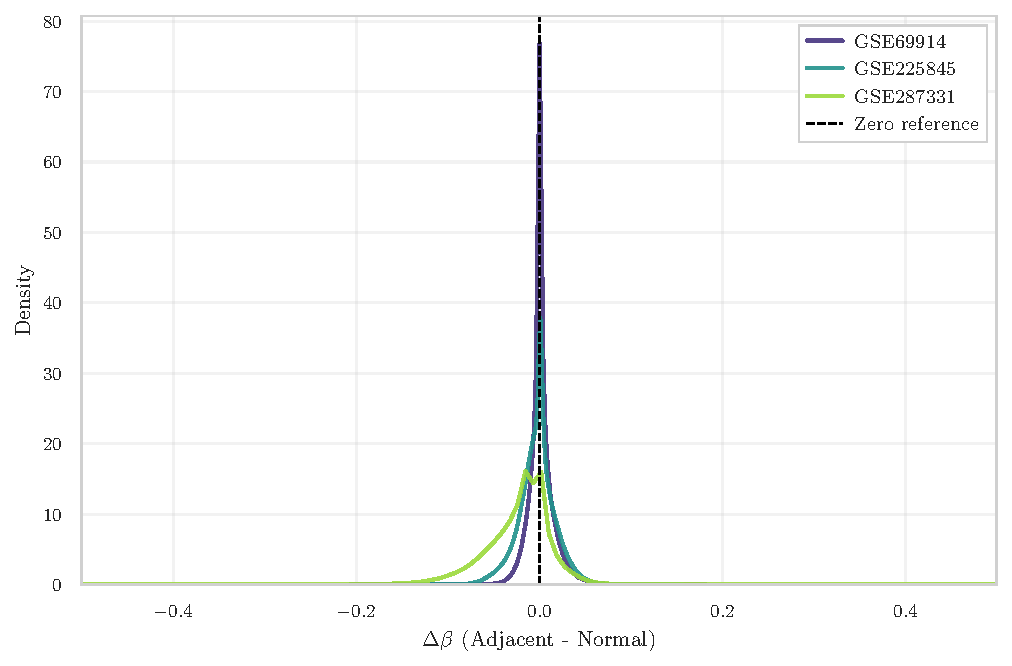
\includegraphics[width=0.5\textwidth]{images/cap3/GSE69914_GSE225845_GSE287331_01_delta_beta_AminusN_overlay_three.pdf}
    \caption{Overlay of $\Delta\beta$ (Adjacent--Normal) density curves 
across the three datasets, computed on the 326{,}330 CpG sites shared 
by all cohorts.}
    \label{fig:delta_density_three}
\end{figure}


\paragraph{Pairwise $\Delta\beta$ concordance across datasets}

To assess whether locus-specific A--N shifts replicate across cohorts, 
pairwise scatterplots are shown for all dataset pairs 
(Figure~\ref{fig:scatter_69914_287331}, 
Figure~\ref{fig:scatter_69914_225845}, 
Figure~\ref{fig:scatter_287331_225845}).  
Each point corresponds to a CpG in the three-way intersection; axes represent 
the mean $\Delta\beta$ (A--N) computed independently within each dataset. Across all pairs, Spearman correlations remain weak ($\rho = 0.05$--$0.29$), 
consistent with the well-established difficulty of achieving 
single-CpG reproducibility across independent methylation studies 
\cite{zhou2017, Fortin2014_funnorm, Leek2010_BatchEffects}.  

The comparison between GSE69914 and GSE225845 exhibits mild monotonic agreement, 
whereas pairs involving GSE287331 show near-zero correlation.  
These results indicate that while the \emph{global} N--A drift remains 
consistent across cohorts (as demonstrated by the density curves), 
\emph{fine-scale, CpG-specific} effects are strongly influenced by 
platform architecture, batch structure, and study-specific variability 
\cite{pidsley2016, Fortin2014_funnorm}.

\begin{figure}[t]
    \centering

    % -------- Subfigure (a) --------
    \begin{subfigure}[t]{0.31\linewidth}
        \centering
        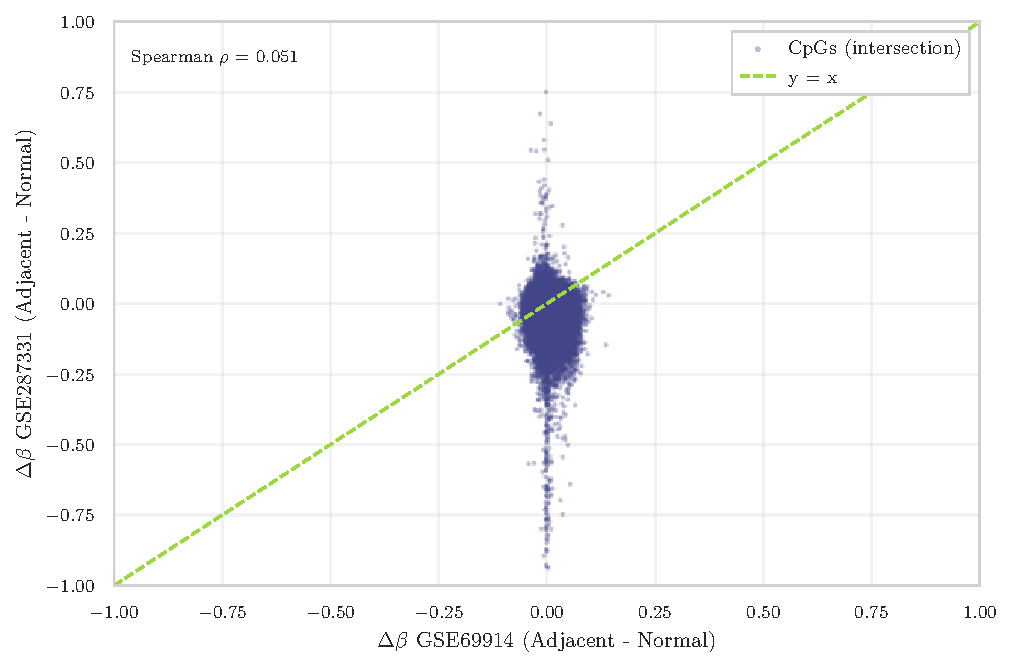
\includegraphics[width=\linewidth]{images/cap3/GSE69914_GSE225845_GSE287331_03_delta_beta_scatter_GSE69914_vs_GSE287331_Adjacent_minus_Normal.pdf}
        \caption{GSE69914-GSE287331, Spearman $\rho \approx 0.051$}
        \label{fig:scatter_69914_287331}
    \end{subfigure}
    \hfill
    % -------- Subfigure (b) --------
    \begin{subfigure}[t]{0.31\linewidth}
        \centering
        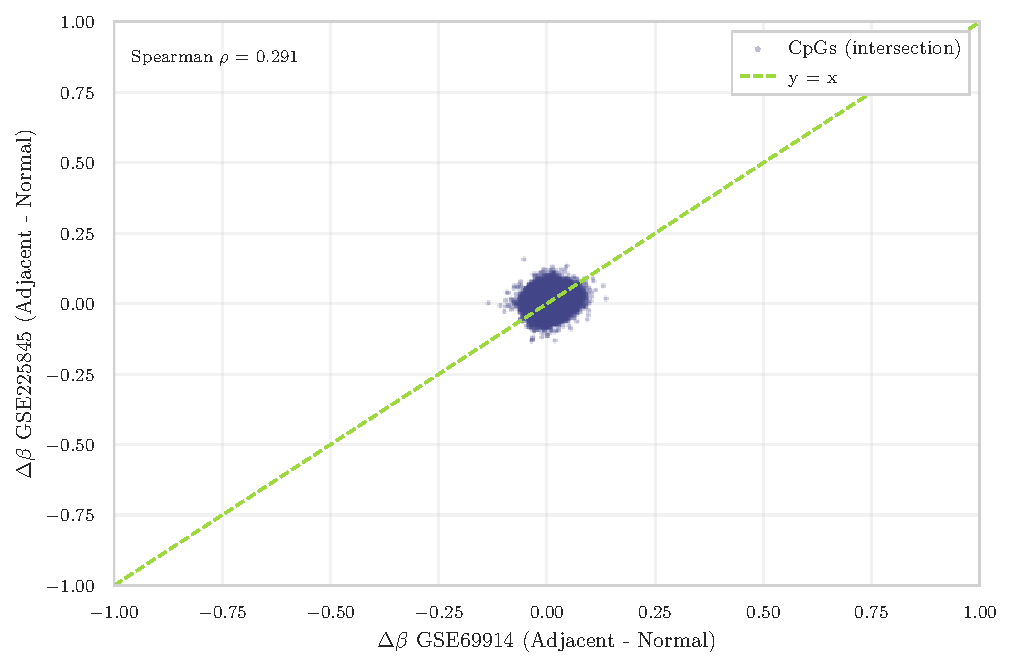
\includegraphics[width=\linewidth]{images/cap3/GSE69914_GSE225845_GSE287331_02_delta_beta_scatter_GSE69914_vs_GSE225845_Adjacent_minus_Normal.pdf}
        \caption{GSE69914-GSE225845, Spearman $\rho \approx 0.291$}
        \label{fig:scatter_69914_225845}
    \end{subfigure}
    \hfill
    % -------- Subfigure (c) --------
    \begin{subfigure}[t]{0.31\linewidth}
        \centering
        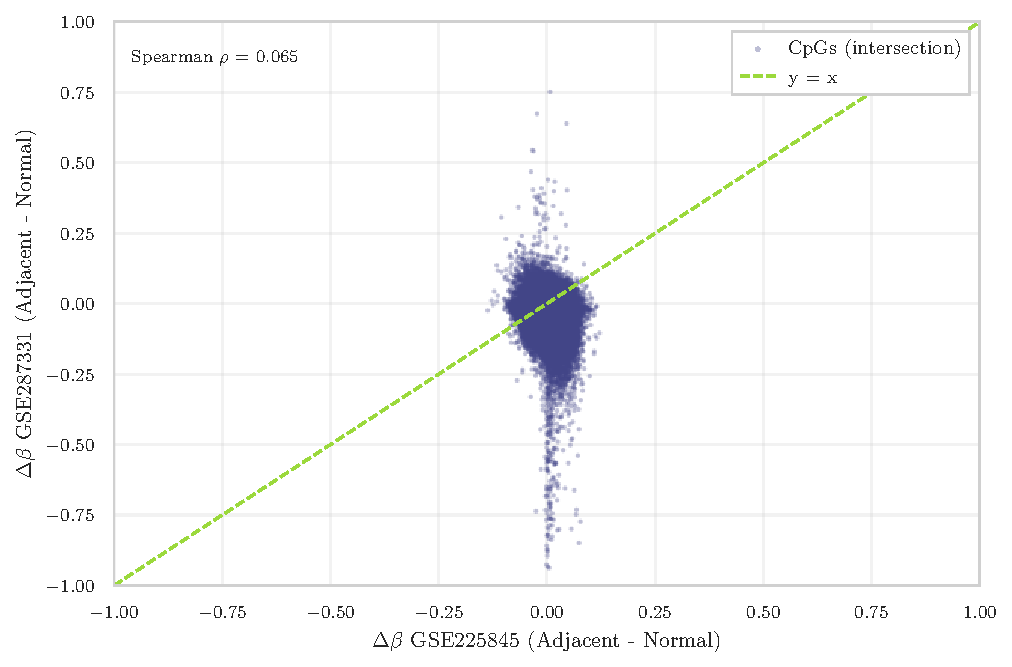
\includegraphics[width=\linewidth]{images/cap3/GSE69914_GSE225845_GSE287331_04_delta_beta_scatter_GSE225845_vs_GSE287331_Adjacent_minus_Normal.pdf}
        \caption{GSE225845-GSE287331, Spearman $\rho \approx 0.007$}
        \label{fig:scatter_287331_225845}
    \end{subfigure}

   \caption{
Pairwise $\Delta\beta$ (Adjacent--Normal) scatterplots across the three 
methylation datasets, computed on the 326{,}330 shared CpG sites.  
Spearman $\rho$ values are reported in each panel.
}
    \label{fig:inter_scatter_three}
\end{figure}



\paragraph{t-SNE embeddings on the shared CpG intersection}

To investigate the multivariate structure of the N--A contrast across 
cohorts, t-SNE embeddings are computed on M-values restricted to the  shared CpGs.  
Two complementary visualisations of the embedding are provided in 
Figure~\ref{fig:tsne_dataset_NA} (coloured by dataset) and 
Figure~\ref{fig:tsne_group_NA} (coloured by tissue state).

When coloured by dataset, the embedding exhibits clear clustering by study, 
reflecting the dominant influence of batch and platform effects in 
high-dimensional methylation data 
\cite{Fortin2014_funnorm, Leek2010_BatchEffects}.  
This pattern indicates that the global methylation structure is largely 
driven by inter-cohort variability, supporting the decision not to merge 
datasets at the raw feature level.

When coloured by tissue state (Normal vs.\ Adjacent), no global separation 
across cohorts emerges, as the embedding remains primarily structured by dataset identity. 
However, within individual study-specific clusters, a state-dependent displacement becomes visible. 
This separation is particularly evident in GSE287331, where Normal and Adjacent samples 
form more clearly distinct substructures. 
This behaviour is consistent with early, localised methylation drift, 
mirroring the quantitative metrics reported in 
Table~\ref{tab:inter_summary_NA}.
\begin{figure}[t]
    \centering

    % -------- Subfigure (a): t-SNE by dataset --------
    \begin{subfigure}[t]{0.48\linewidth}
        \centering
        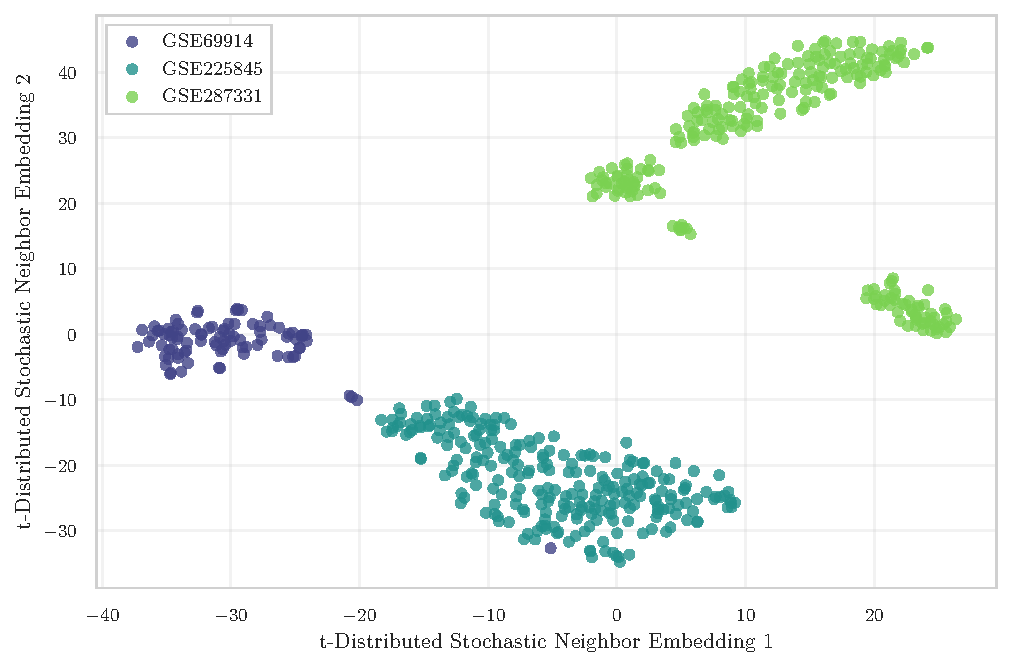
\includegraphics[width=\linewidth]{images/cap3/GSE69914_GSE225845_GSE287331_07_tsne_by_dataset_NA.pdf}
        \caption{t-SNE coloured by dataset \\$\text{trustworthiness}=0.976$}
        \label{fig:tsne_dataset_NA}
    \end{subfigure}
    \hfill
    % -------- Subfigure (b): t-SNE by group --------
    \begin{subfigure}[t]{0.48\linewidth}
        \centering
        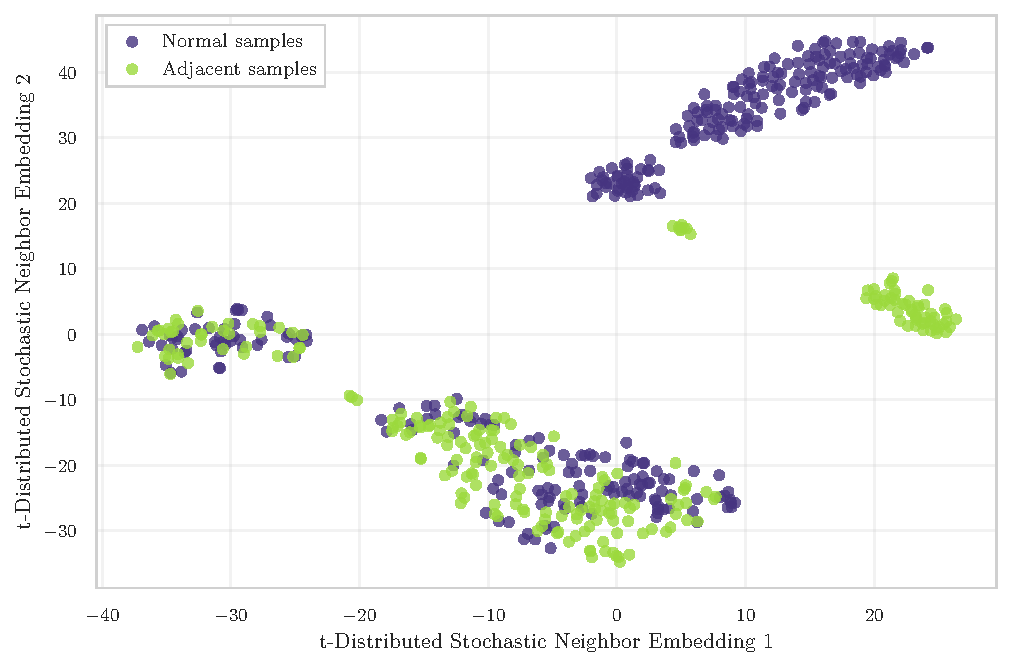
\includegraphics[width=\linewidth]{images/cap3/GSE69914_GSE225845_GSE287331_08_tsne_by_group_NA.pdf}
        \caption{t-SNE coloured by tissue state \\$\text{trustworthiness}=0.976$}
        \label{fig:tsne_group_NA}
    \end{subfigure}

    \caption{
t-SNE embeddings computed on the 326{,}330 CpGs shared across GSE69914, 
GSE225845, and GSE287331. 
}
    \label{fig:tsne_two_views}
\end{figure}


Overall, the visual analyses corroborate the quantitative metrics: early 
epigenetic drift is detectable in all cohorts, but its magnitude and 
visibility vary substantially, with GSE287331 exhibiting the clearest 
field-defect signature.  
The combination of globally subtle yet directionally consistent 
$\Delta\beta$ patterns, weak CpG-level concordance, and 
dataset-specific multivariate structure reinforces the view that the 
Normal$\rightarrow$Adjacent transition reflects genuine early 
epigenetic deregulation rather than dataset-specific artefacts.

\section{Exploratory Findings and Pre-Processing Implications}
\label{sec:cap3_conclusions}

The exploratory analyses presented in this chapter reveal a consistent picture 
across all three cohorts: the Normal--Adjacent transition does not manifest as a 
global reorganisation of the methylome, but as a subtle, focal drift that becomes 
detectable only through locus-specific perturbations and multivariate 
displacements. This characteristic makes it particularly sensitive to technical 
sources of variability --- probe-design bias, batch effects, and platform 
differences --- which operate at a comparable or larger scale than the biological 
signal of interest.

This sensitivity has direct methodological consequences. Raw methylation data, 
as distributed via GEO, cannot be used directly for downstream modelling without 
first addressing these technical confounders: doing so would risk attributing 
platform-specific artefacts to genuine epigenetic alterations, or conversely, 
suppressing the subtle Normal--Adjacent differences under overly aggressive 
normalisation. The challenge is therefore not simply to clean the data, but to do 
so in a way that preserves the biological structure identified here.

Chapter~\ref{chap:data_preprocessing} addresses this challenge by developing a structured, platform-aware 
preprocessing pipeline. Each step is motivated by the specific limitations 
identified in the present chapter.